\documentclass[12pt, a4paper]{report} % for a short document
\usepackage[english]{babel}
\usepackage{blindtext}
\usepackage [vscale=0.76,includehead]{geometry}              
\usepackage{fullpage}
\usepackage{subcaption}
\usepackage{mathptmx} % font = times
\usepackage{helvet} % font sf = helvetica
\usepackage[latin1]{inputenc}
\usepackage{relsize}
%\setsecnumdepth{subsection}
\setcounter{secnumdepth}{3}
\usepackage{tocloft}
%\def\cftchapteraftersum{.}
\oddsidemargin 0.0cm  
\evensidemargin 0.0cm  
\textwidth 17cm 
%\topmargin -1cm 
\textheight 23.5cm
%\addtolength\headheight{16pt} 
\usepackage{graphicx}
\usepackage{float} 
\usepackage{multimedia}
\usepackage{amsmath,amssymb}
\usepackage{listings}
\usepackage{graphicx} % Allows including images
\usepackage{booktabs} % Allows the use of \toprule, \midrule and \bottomrule in tables
%\usepackage[nottoc, notlof, notlot]{tocbibind}
\usepackage{amsfonts}
\usepackage{amsmath,bm}
\usepackage{hyperref}
\usepackage{cite}
\lstset{
  numbers=left,   
  firstnumber=1,
  numberfirstline=true,
  language=C, 
  frame=L
  } 
%\pagestyle{book}
\bibliographystyle{plain}

\begin{document}
\selectlanguage{english}



\chapter*{Abstract}

This thesis addresses the problem of restoring the complete history of a 2D geological 
subsurface also called a cross-section \cite{BalancedCrossSections}. It is a key problem for geologists when they want to understand how the terrain transformed to be in state it is today. Moreover restoring cross section allows them to date geological events such as faults, erosion or sedimentation. It is also a major source of interest for oil searchers who can identify places where oil is likely to be trapped in by looking at the cross section evolution. Tools to tackle this problem have already been created and can  be categorized into two kinds: geometrical based tools which deform the initial cross-section relying only on geometrical and kinematical property of the drawing and physical based ones which focus on runninng a simulation using physical equation applied to the section in order to deform it. However those tools usually restore only one scenario of the cross-section history when several of them can exist.\\\\
 Here, we propose a new hybrid method which focuses on proposing multiple scenarios of the cross section restoration. As an input we take a cross section drawing containing topological data and we map a mass spring system on it, which is the center of our animation process. In addition we propose to the user to choose among possible events to transform the cross section to its restoration state and simulate the selected ones. Each time an event simulation ends, we ask the user to make another event choice until there are no event to propose left. One main feature of our methods is that the user is able to come back to its previous choices and create an other scenario as he pleases in order to build a tree of scenarios labelled as Story Tree.\\\\

\tableofcontents

\chapter{Introduction}
\label{ch:intro}
Hand-drawn sketches are highly used in geology for illustrating and validating hypotheses. It is the main way of keeping and showing geological data. Indeed, showing an image of what we have in mind is a really powerful way to convey our thoughts, especially here in geology where we can draw from multiple points of view (top view or side view in general). Futhermore geologists write many anotations on their drawing to give more hints and be more specific in the information they want to show in their sketches.\\\\
For instance sketches can be used to reconstruct a 3D view of the subsurface by drawing a 2D top view of the current terrain \cite{brazil} and using anotations or to represent 2D vertical cross-sections. \\\\
However anotations are limited in explaining what happened in the past, it is difficult to anotate the past of the geological representation on a single sketch. Therefore geologists must draw several sketches when they whant to show the history of a terrain. \\\\
This is the case when they build cross section restoration \cite{SectionRestoration}. It consists in drawing several sketches of the same cross section at different time steps starting from its current state. A cross section is composed of several geological elements, in particular blocks, layers and faults. The layers they draw correspond to different sedimentary layers that have deposited  along history. Blocks correspond to parts of the section which are between two faults or one fault and on boundary of the sketch. They contain part of layers which have been cut by faults and are called geological unit (unit for short).
Finally faults correspond to breaks in the section and create discontinuities in it. They can be of three types:
Normal, Reverse or Strike-slip. Normal and Reverse faults correspond to vertically oriented breaks which make blocks slide among their left or right side. Normal faults happen during extension while reverse faults happen during compression. As for Strike-slip faults, their are horizontal breaks that make blocks sliding on their bottom or upper parts.\\
However as we are in the 2D vertical case we are only interesed in the reverse and normal faults.\\\\
Figure ~\ref{geostruct} summerize the cross section structure and Figure ~\ref{crossxeg} show an example of a cross section.
 \begin{figure}[H]
	\centering
	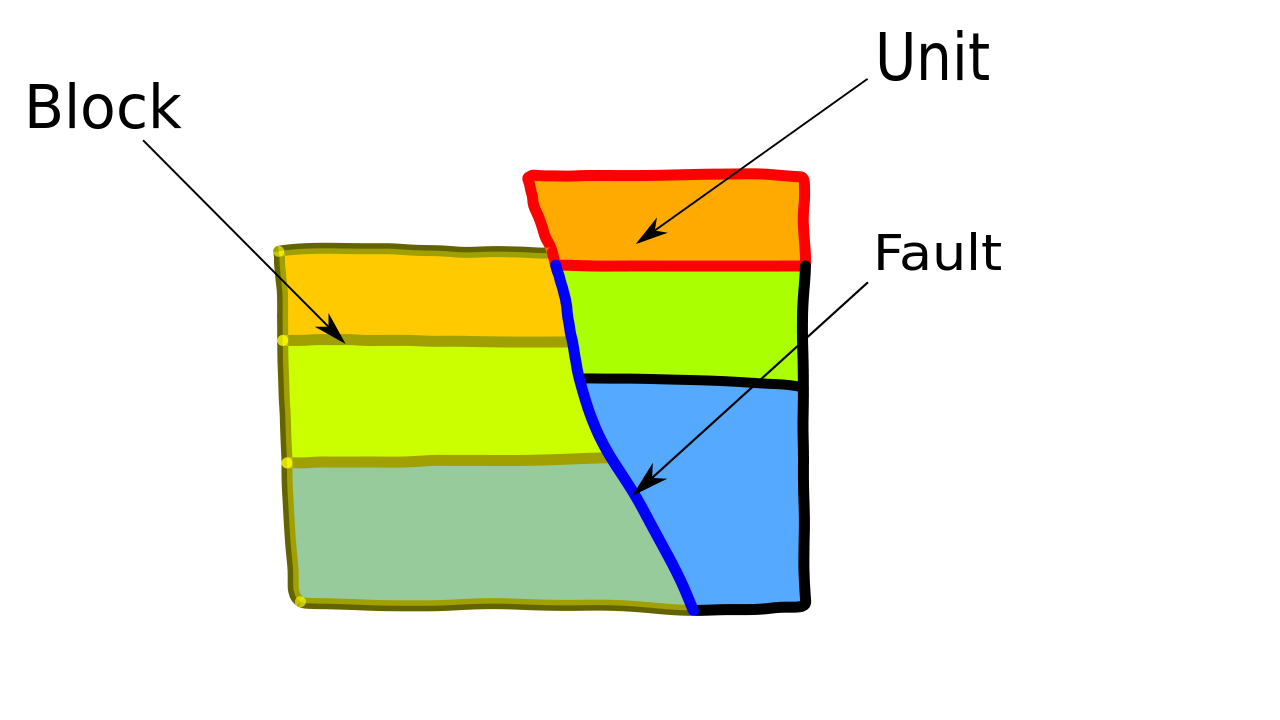
\includegraphics[scale=0.3]{geologyStructEdit.png}
	\caption{Cross section structure}
	\label{geostruct}
\end{figure}

\begin{figure}[H]
	\centering
	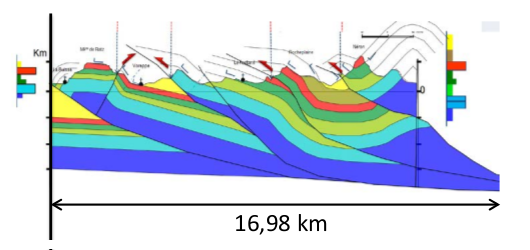
\includegraphics[scale=0.8]{Wraped_Section.png}
	\caption{Chartreuse Cross Section}
	\label{crossxeg}
\end{figure}

The current state of the cross section is the result of several geological phenomena such as erosion, foldings, sedimentations, or fault impacts, which occured in the past at different time. Consequently, restoring a cross section can differ depending on the geologists' point of view.\\\\
However using the initial sketch  and geometrical tools like \cite{Move}, geologists are able to draw the past state of the cross section before any erosion, fault and sediment events. Thus they obtain a restoration which is usually unique and doesn't differ much between geologist. 
Most of the time, an analysis of the different layers and faults usually lead to the same geometrical evolution reconstruction which has been provoqued by compression or extension of the rock masses before, after or during deposit and erosion of the sediments and basement rocks. \\\\
Consequently the main problem geologist are facing in this restoration is to find what really happened between the current state to the past one. They have two main problems to solve. First they have to find all the events that occured from the past to the current state. Then they have to find they occurrence order because it is possible that by changing the event order we obtain the same restoration at the end. Futhermore it is possible to find the same restoration having identifying different events in two different hypothesis. \\\\
Consequently geologists have to draw many sketches in order to expose their hypothesis. In addition those drawings are rather limited: on top of representing only one 2D cross-section of the terrain being investigated, they can only represent hypotheses on the underground geometry at discrete time steps, rather than a complete continuous history. Futhermore insuring consistency between these sketches over time heavily depends on available data, maturity of the regional geological interpretation and the skills of the geologist, i.e. his knowledge on the way rocks and sediments fold, on the way faults propagates and produce sliding and displacements, and on the way sediments are deposited or eroded, etc...\\\\
Recently, it was proposed to organize geological sketches into story trees to present and compare different interpretations of the formation of a given terrain \cite{lidal} but the task remains labor-intensive, requiring the geologist to draw every sketch in the story tree. Moreover, even while being skillful and experienced, it is hardly impossible for a geologist to express a continuum of the deformation of a geological cross-section with available tools.
In this internship, we would like to follow up on this line of research by proposing methods for inferring a geological story tree directly from one geological sketch, and presenting the resulting tree of possible geological stories as an animation.\\\\

\chapter{State of the Art}\\

Several solutions of very different kinds have been proposed to solve the problem of correctly exposing many restoration hypothesis without inconsistencies and without spending too much time creating them. We distinguish three main types of methods: geometrically based, physically-based and sketch-based ones.\\\\
Geometrical methods consist in assuring only geometric consistency when exposing the solution while mecanical ones consist in running a physical simulation over the past cross section and see if the animation created confirm the restoration process hypothesis. Finally sketch based methods , which are more recent, propose geologist to optimise the number of need sketch for obtaining a restoration by storing them in a story tree structure.\\\\

\section{Geometrically-based methods}

Geometrically-based methods are usually interactive process where the user will restore the cross section by either flattening layers, moving blocks and removing or adding matter.
Those methods are widelly used by geologists because they gives them a large control over the restoration process while keeping the geologic and geometric consistency of the section.  The deformation process is done by applying  kinematic algorithms on the different block and unit. Futhermore those methods are able to take into account a wide range of geological phenomena such as compaction, erosion, sedimentation, folding but also more specific effects such as thermal subsidence and isostasy (crust floating on the mantle) for finner restoration results. In addtion, the kinematic algorithm used in the restoration process produce real time rendering which is why these methods are able to be interactive.
Figure ~\ref{mve} shows a portion of the geometric restoration process using the "Move 2D" tool \citep{Move}:

\begin{figure}[H]
	\centering
	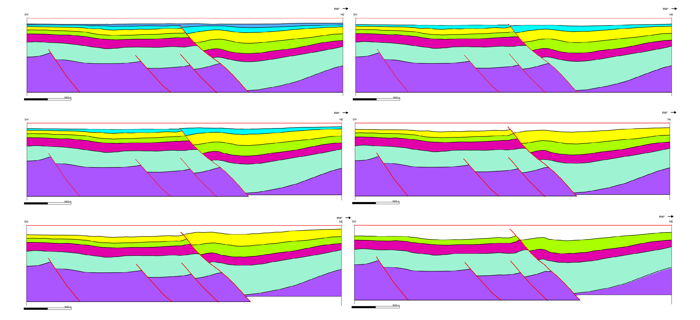
\includegraphics[scale=3]{mve2D.png}
	\caption{MVE 2D restoration sequence}
	\label{mve}
\end{figure}

In addition this kind of method can produce forward modeling animation which can help geologists to validate their hypothesis in the case they want to check if the restoration they produced matches the input cross section. Futhermore they can consider the 3D aspect of a subsurface using several cross sections and a 3D model of the considered area like shown in Figure ~\ref{mve3}.

\begin{figure}[H]
	\centering
	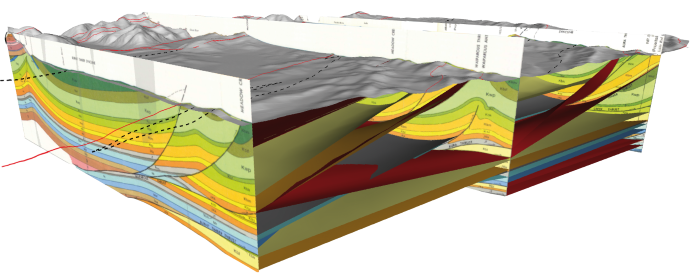
\includegraphics[scale=1]{mve3D.png}
	\caption{MVE 3D. 3D modeling using several 2D cross sections}
	\label{mve3}
\end{figure}


The main drawback of these methods is their lack of physical realism which can be noticable and inconvenient for some restoration.
\section{Phycally-based methods}
Phycally-based methods run mecanical simulations over cross sections to animate them. Most oft the time they are fully automatic methods with very few interactions with the user. They are based on the Coulomb theory which describe how layers will react to contact and stress coming from  adjacent layers. Moreover it describes how a block will slide while being submitted to forces and stress. In addition they also use a material deforming and breaking method caracterized by the Young Modulus parameter which give breaking condition of materials. \\
As those methods are fully automatic, they are easier to use and are handier for geologists.
We can distinguish two types of physycally based methods: forward simulation and backward simulation ones.
The two methods use finite elements methods to run their simulation but take a different approach of the restoration problem.
\subsection{Forward physics simulation methods}
Forward simulation methods propose to run the simulation over the restoration, which has been provided by any arbitrary means, and see if it matches (not necessarily perfectly) the current cross section. They simulate folding forces and create fault where materials are supposed to break. Other geological events such as erosion, sedimentation or compaction are also taken into account. Figure ~\ref{slam} shows a simulation run with SLAMTec \cite{SLAMTec} which implement forward simulation:

\begin{figure}[H]
	\centering
	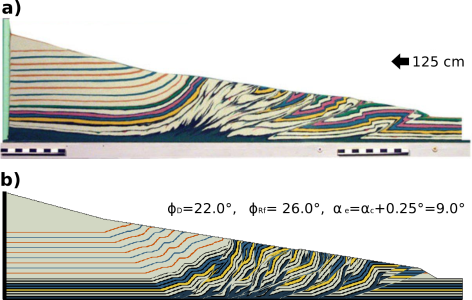
\includegraphics[scale=0.5]{slamtec.png}
	\caption{Slamtec cross section modeling}
	\label{slam}
\end{figure}
We can note that similar result can be obtained with other forward simulator such as OptumG2 \cite{Optum}
\subsection{Backward physics simulation methods}
Backward simulation methods propose the same kind of simulation than forward simulation but change the way the geological events occur. They propose to run a mecanical simulation on the starting cross section and apply forces and conditions opposed to the true event impacts that have been applied. For instance if the current section has been subject to compression forces the method will apply extension forces to the model instead. The same process is repeated for un-doing other types of geological events\\\\
 Figure ~\ref{dyn2} shows a restoration example simulated with "Dynel 2D" \cite{Dynel} which implements this method:
 \begin{figure}[H]
	\centering
	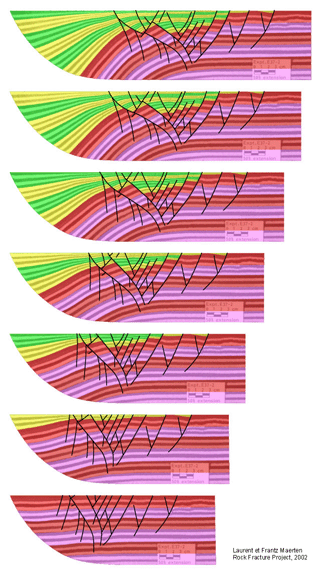
\includegraphics[scale=0.6]{dynel2D.png}
	\caption{Dynel 2D restoration sequence}
	\label{dyn2}
\end{figure}

 While this method is likelly to produce much better results that forward method in terms of similarity with the restoration and the current state of the section, it is more difficult to use because there exist many uncertainties on identifying the events that occured between the two states.


Even though physically based methods respect physic laws and produce very consistent results, they are not perfectly matching the cross section current state and the restoration. Thus they cannot fully validate the hypothetical section history they have simulated. In addition, depending on the physical model accuracy used in the simulation, the computation time can take up to several hours.

\section{Sketch based methods}

Stetch based methods , which are more recent, try to bring back the traditionnal way of restoring cross section by organising geologist drawings into trees.
Like mentionned in the introduction, Lidal \cite{lidal} proposed a solution using story trees to organize geologists' reasoning. Starting from the initial drawing (and node of the tree), the geologist can draw several stories where each node of the tree conctains a new sketch. In addition it is possible to superimpose the previous drawings to the new one, helping keeping geometrical consitancy and reducing conciderably the time spent for creating a sequence. Futhermore as geologists use mainly seismic recordings to draw their starting sketch, the method allow them to display this inital recording in background, helping them in being more conherent.\\\\
 As a result with fewer sketches and less time spent drawing, geologists can express their ideas better than with traditionnal sketching. Futhermore this method is really efficient when exploring different hypothesis  because at each node geogist can create another branch to explore a new possibility for either refining their animation or trying different scenarios. Figure ~\ref{lidal} shows an example of Lidal methods:\\\\
 \begin{figure}[htb]
\centering
\begin{tabular}{@{}cc@{}}
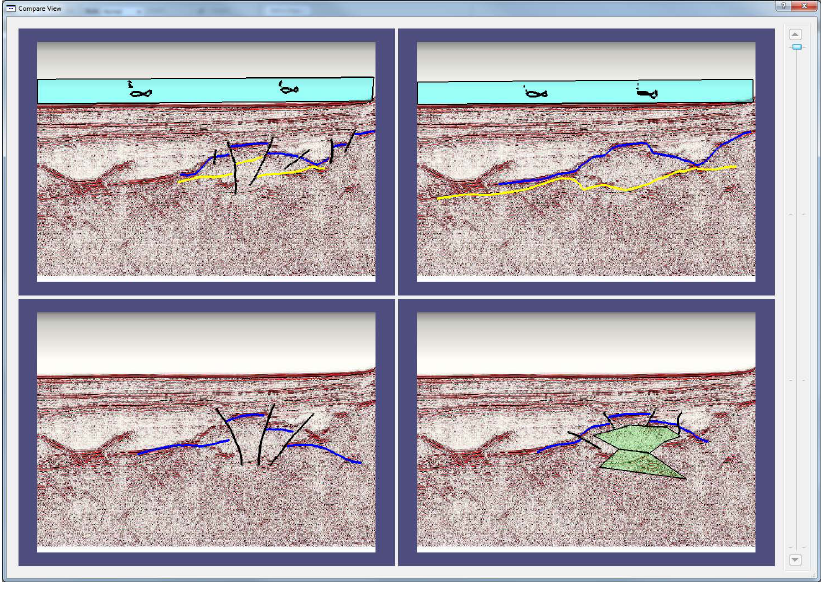
\includegraphics[width=.35\textwidth]{lidal0.png}&
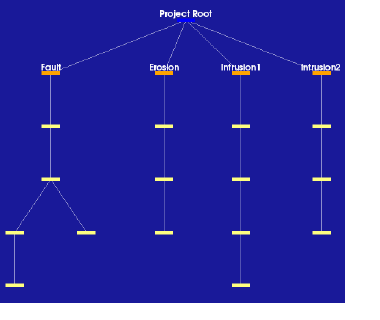
\includegraphics[width=.35\textwidth]{lidal1.png}\\
\end{tabular}
\caption{Lidal sketch based method example.}
\label{lidal}
\label{unerodeeg}
\end{figure}
However this method doesn't necessarely keep the topological conherence of the drawings unless the geologist spend more time being carefull of maintaining it through their sequence. This topological aspect should not be ignored be cause it can refut hypotheses when dealing with very old cross sections where the terrain's topology underwent drastic changes.\\\\\

In our project, we propose an hybrid method combining features of the three kinds of methods we just reviewed.
\chapter{Overview of our solution}

In this thesis we contribute in the cross-section restoration field by proposing a new method based on multiple scenarios exploration and animation. Our method consist in un-doing geological event sequences that occured in a cross section and proposing several restoration scenarios.\\\\

Our approach works as follows: we first proceed to a sketch analysis where we detect most of the geological events that occured in the cross section and organise them into an Event Graph (see section ~\ref{sub:storytel}).
Next we sort those events using time dependencies and probability of occurrence, and we start an interactive recursion where the geologist can choose events that need to be un-done. Then our system runs a backward simulation which attempts to undo the selected events. Afterwards the user can accept or backtrack the simulation and we continue this process until obtaining the desired restoration where no more events are to be un-done.
Finally, when the geologist found his restoration sequence, he can play it in reverse to show a forward animation of the recovered cross section's history.

During the project, we were motivated by restoring the Charteuse cross-section which has been provided by geologists with its restoration. As geologists can evaluate each scenario animation we can simulate, it is a good example for validating and showing the efficiency of our method.\\\\
Thus we wanted to provide backward simulations of several interactively created scenarios inbetweening the current Chartreuse section and its restoration. Running this cross section in our interactive recursion creates several restoration scenarios which we encode into a story tree (see section ~\ref{sub:storytel}) similary to \cite{lidal}. Each path of the tree corresponds to one animation of our inbeteweening and each branch corresponds to the simulation of one or several events. The resulting story tree looks like Figure ~\ref{maingoal}
 \begin{figure}[H]
	\centering
	\includegraphics[scale=0.6]{mainGoal.png}
	\caption{Cross Section Story Telling process on Chartreuse section}
	\label{maingoal}
\end{figure}\\


In our example we can observe several geological events to un-do; we will list them in the following section.
Then we will make an overview of our story telling process and of our animation model. Finally we will review our input data structure and our general workflow

\section{Geological Events List}
Here we present all the geological events we want to un-do in order to restore our cross-section.
We listed at least four events to un-do: erosion, sedimentation, folding and faults. We show for each event an example of un-do.
\subsection{Erosion}
Inside a cross section, erosion impact can be noticed by thickness variation in the same layer.
In many cases it digs cavities capable of dividing units into two parts. Thus, in order to un-do this event we add the lacking matter to the concerned units as shown in Figure ~\ref{unerodeeg} and Figure \ref{unerodecveg}

\begin{figure}[htb]
\centering
\begin{tabular}{@{}cc@{}}
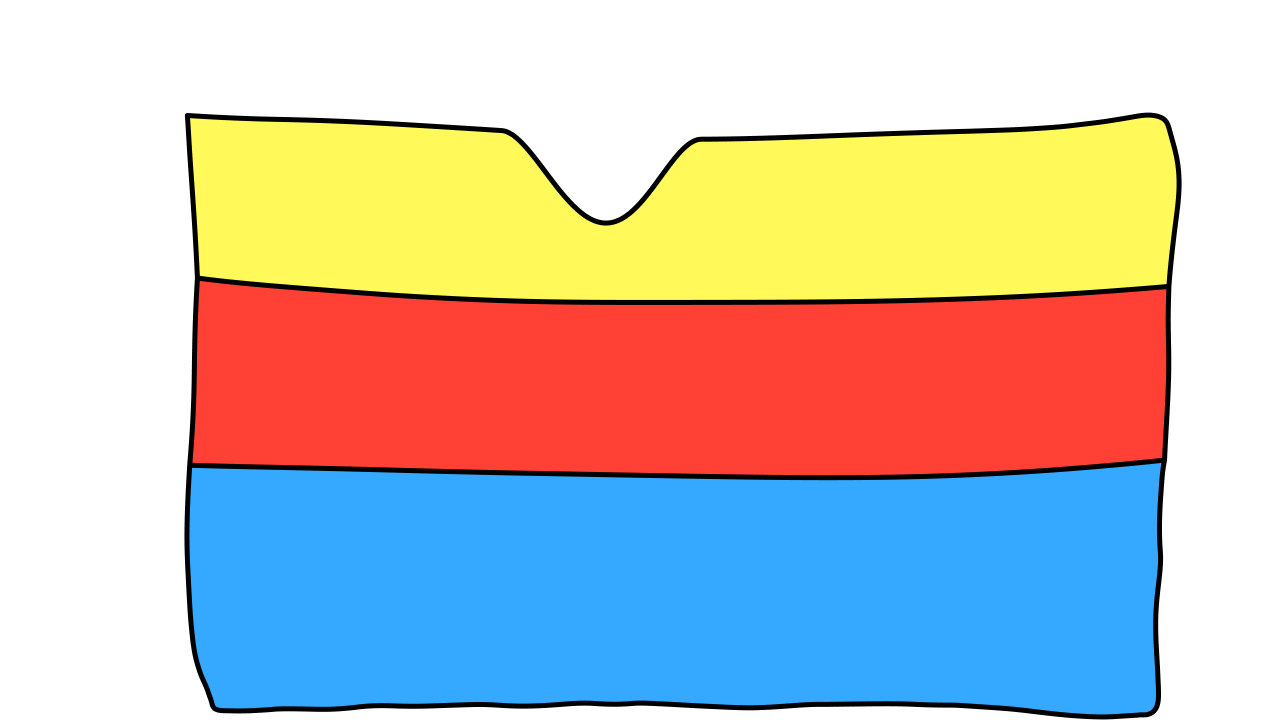
\includegraphics[width=.35\textwidth]{unErodeUpDescription0.png}&
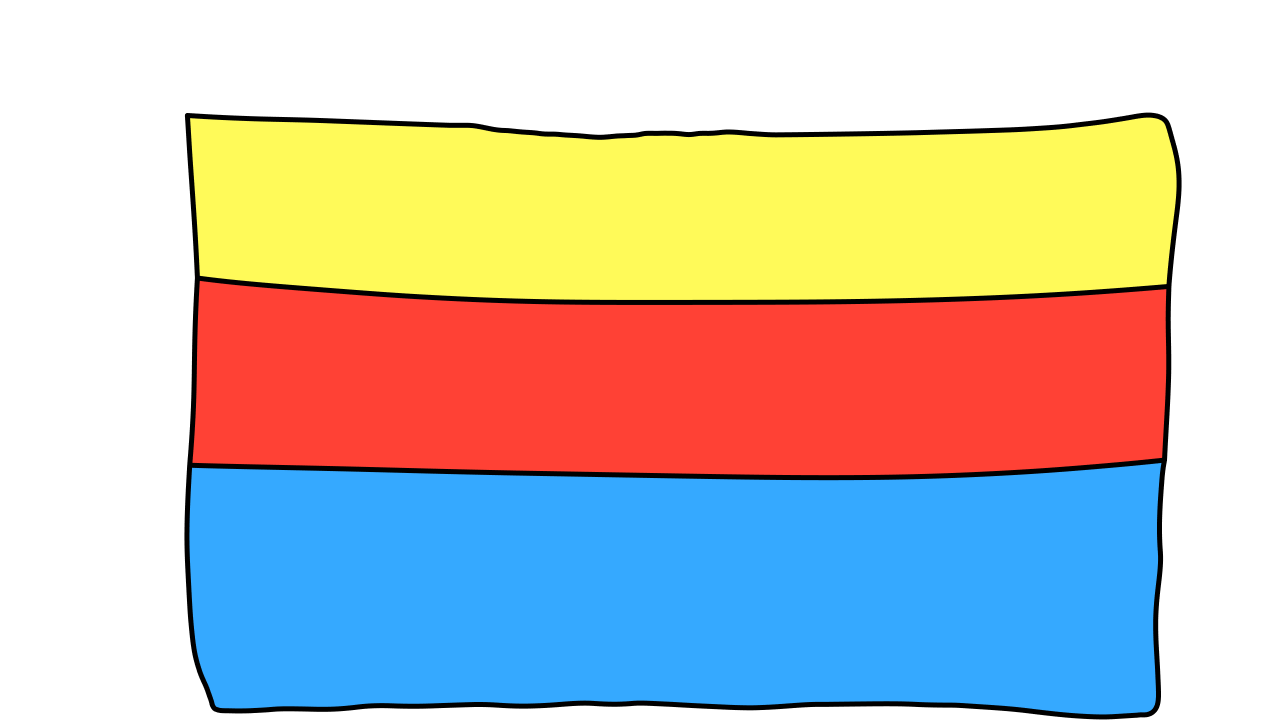
\includegraphics[width=.35\textwidth]{unErodeUpDescription1.png}\\
\end{tabular}
\caption{Un-Erode example of filling a unit cavity.}
\label{unerodeeg}
\end{figure}

\begin{figure}[htb]
\centering
\begin{tabular}{@{}ccc@{}}
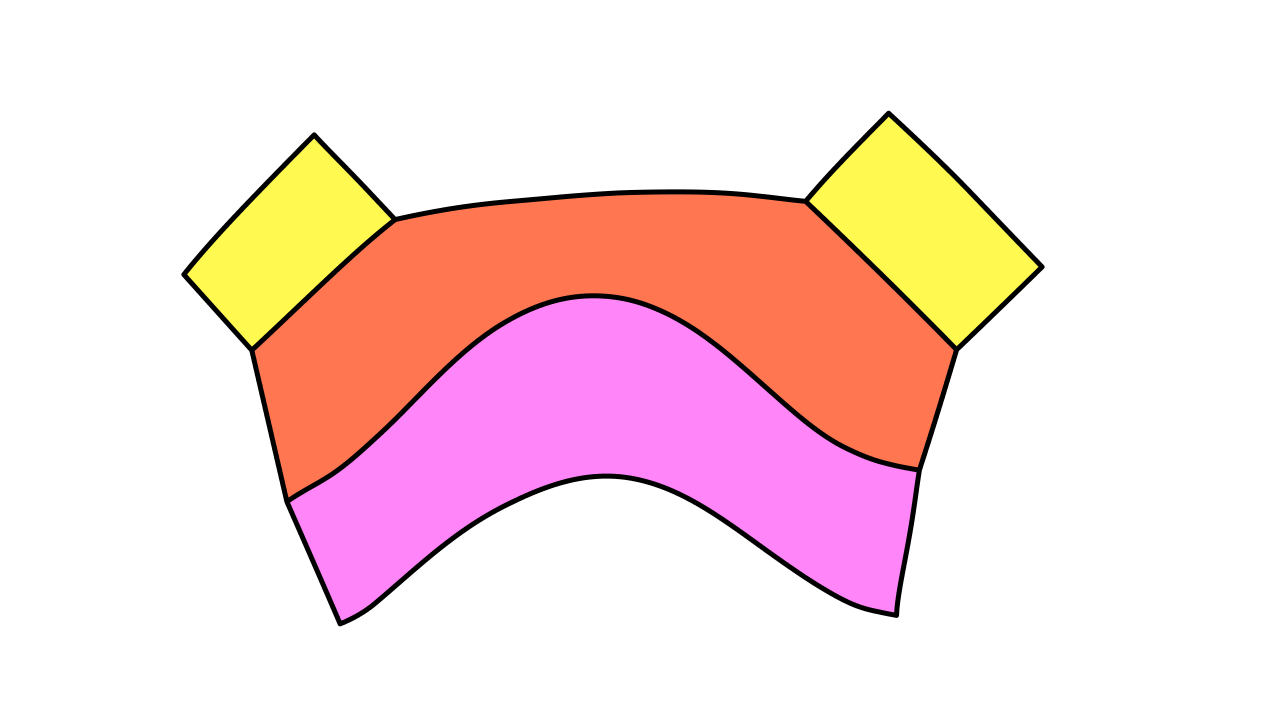
\includegraphics[width=.35\textwidth]{unErodeConvexDescription0.png}&
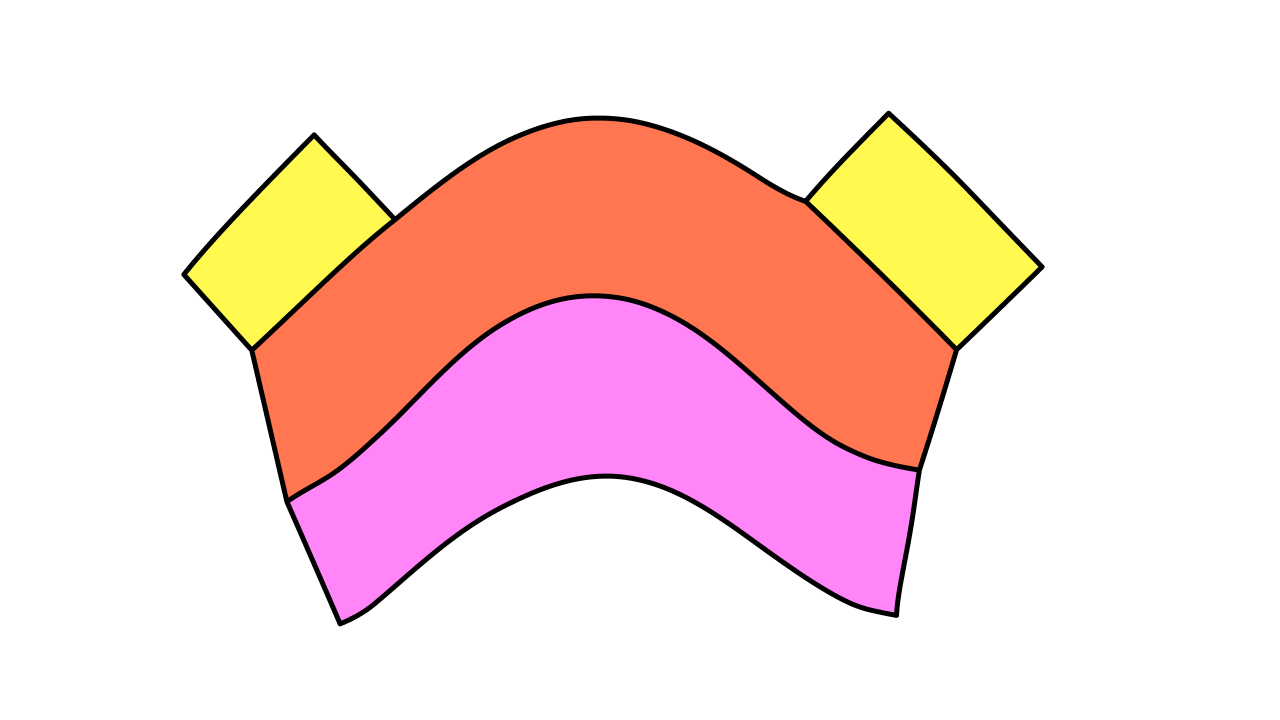
\includegraphics[width=.35\textwidth]{unErodeConvexDescription1.png}&
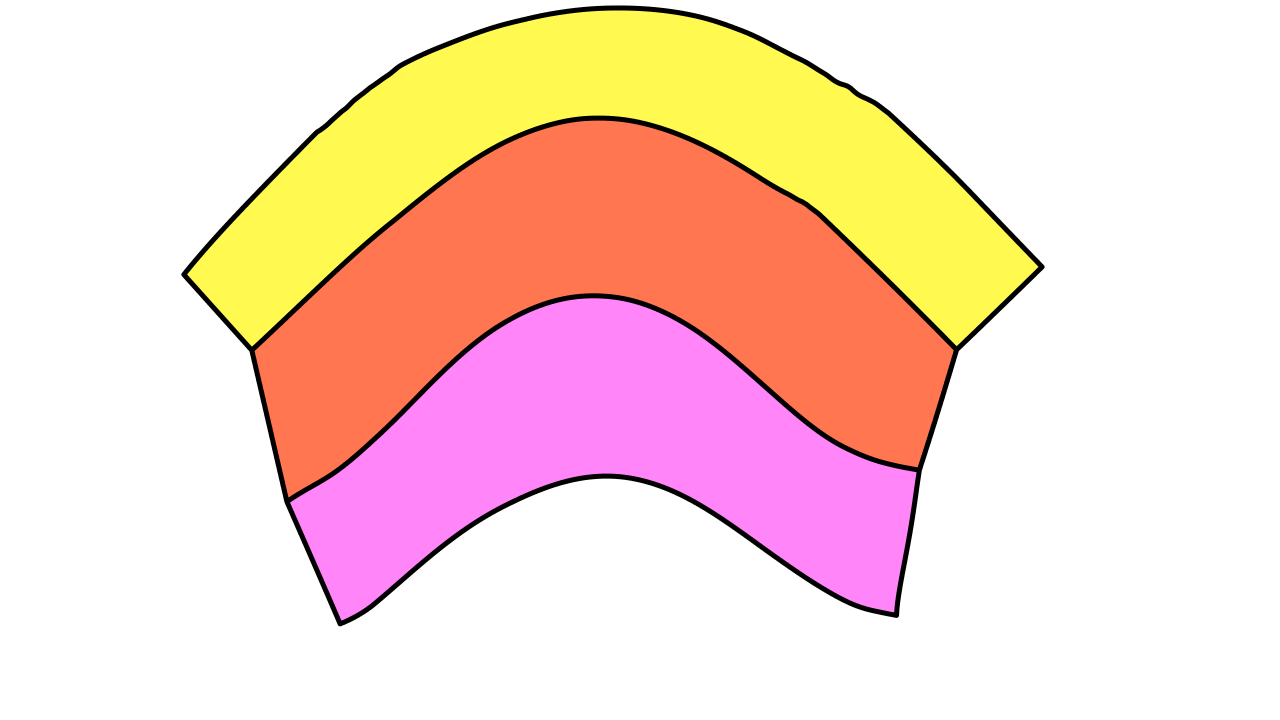
\includegraphics[width=.35\textwidth]{unErodeConvexDescription2.png}\\
\end{tabular}
\caption{Un-Erode example of filling a cavity which erased a unit.}
\label{unerodecveg}
\end{figure}\\\\
The full explanation of the un-doing proccess is explained in section ....

\subsection{Sedimentation}
In geology, sediments are an importants assets for event datation because we know their age accurately. In addition, they always deposit in horizontally regardless of the surface relief. Therefore it is a easy event to un-do because we just have to remove matter progressively and horizontally, the same way as Figure ~\ref{unsedeg}
\begin{figure}[htb]
\centering
\begin{tabular}{@{}ccc@{}}
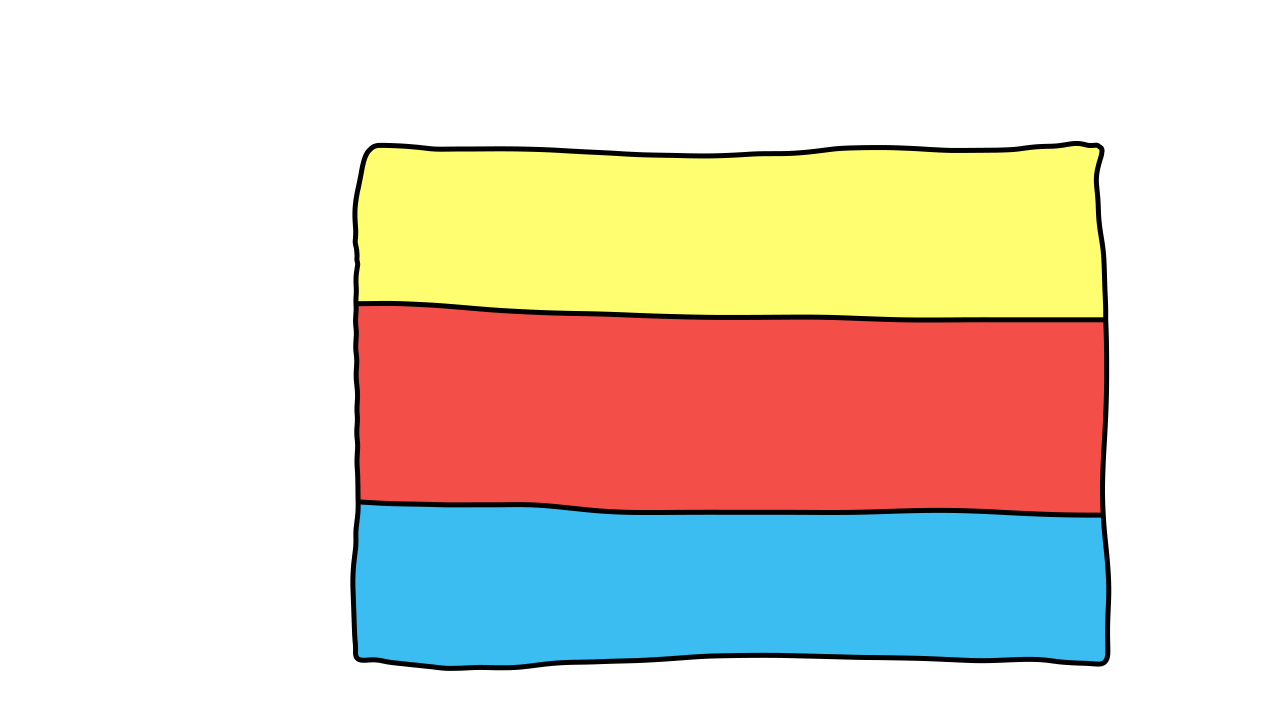
\includegraphics[width=.35\textwidth]{unSedimentDescription0.png}&
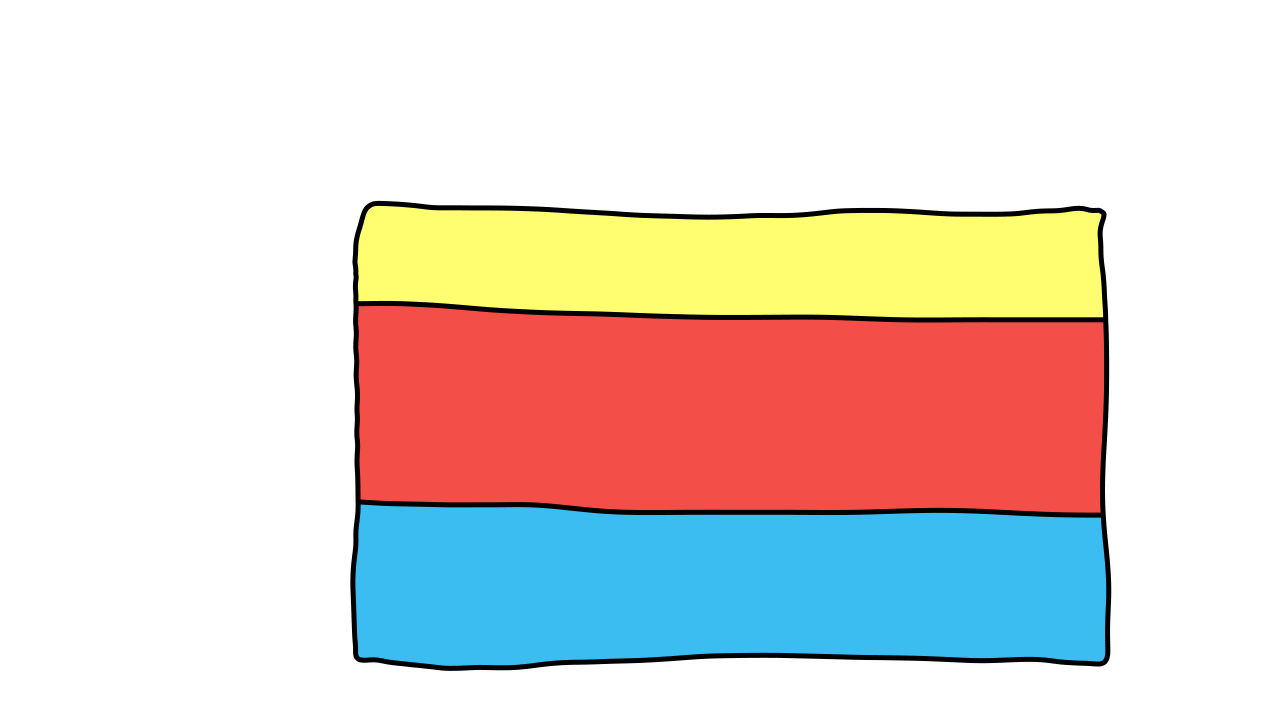
\includegraphics[width=.35\textwidth]{unSedimentDescription1.png}&
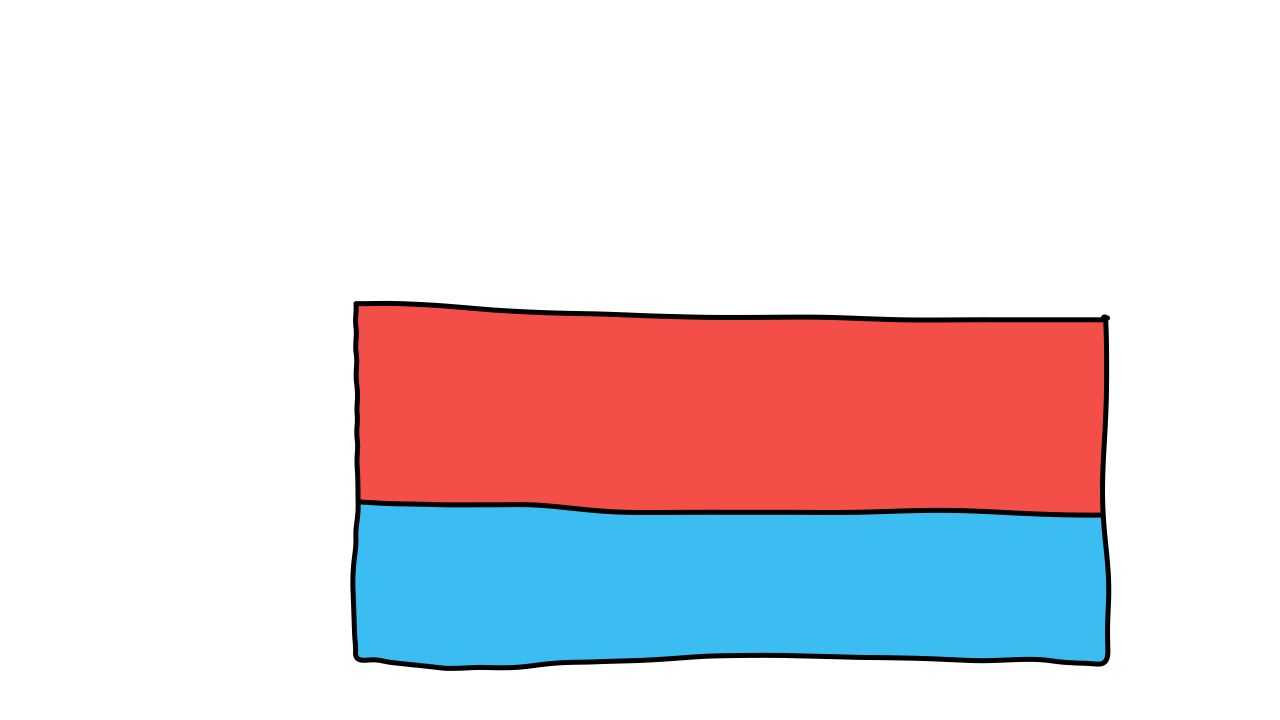
\includegraphics[width=.35\textwidth]{unSedimentDescription2.png}\\
\end{tabular}
\caption{Un-Sediment layer example.}
\label{unsedeg}
\end{figure}\\\\
The full explanation of the un-doing proccess is explained in section ....

\subsection{Folding}
\label{sub:fold}
Through their history, cross sections are submitted to forces resulting either from tectonic movements, compression or extension, or some other kinds of geological events (volcanic activity for instance). Those forces impact cross sections by folding them and sometimes cause breaks inside it (see section ....). Here we are interested in the force process which only fold the cross section and which can be un-did by applying opposite forces to the one that have been applied like in Figure ~\ref{unfoldeg}

\begin{figure}[htb]
\centering
\begin{tabular}{@{}cc@{}}
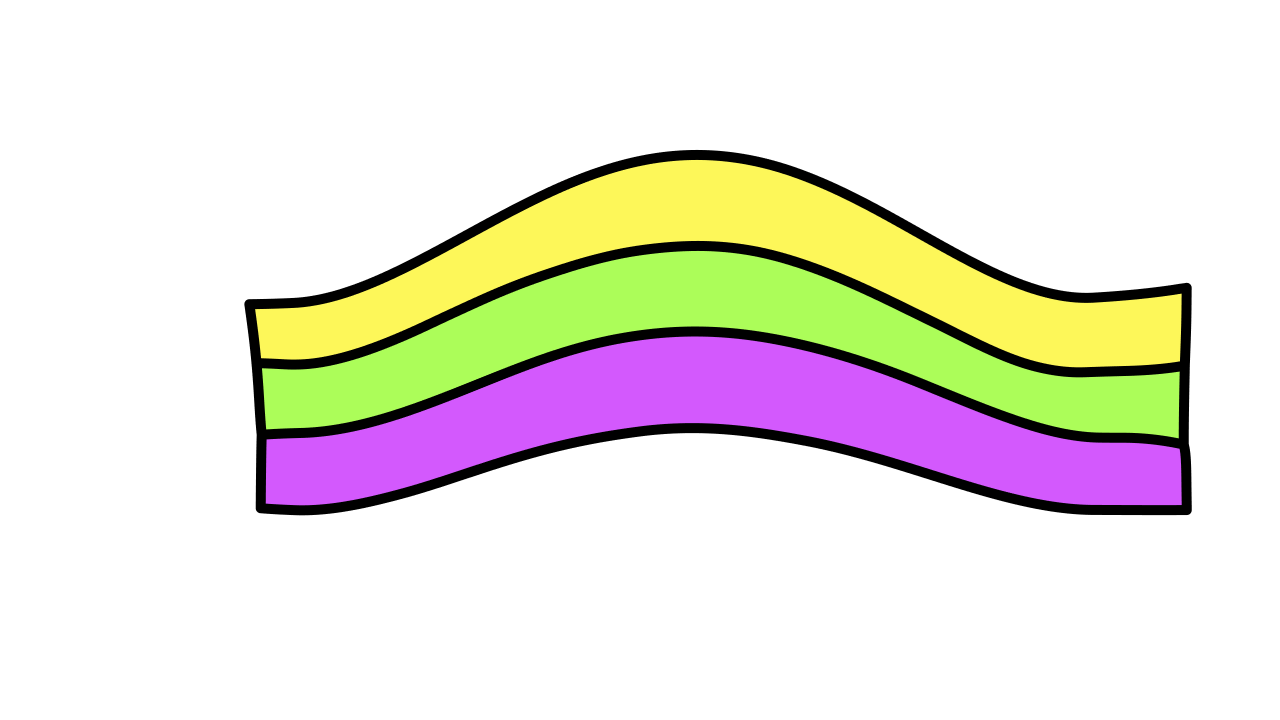
\includegraphics[width=.35\textwidth]{unFoldDescription0.png}&
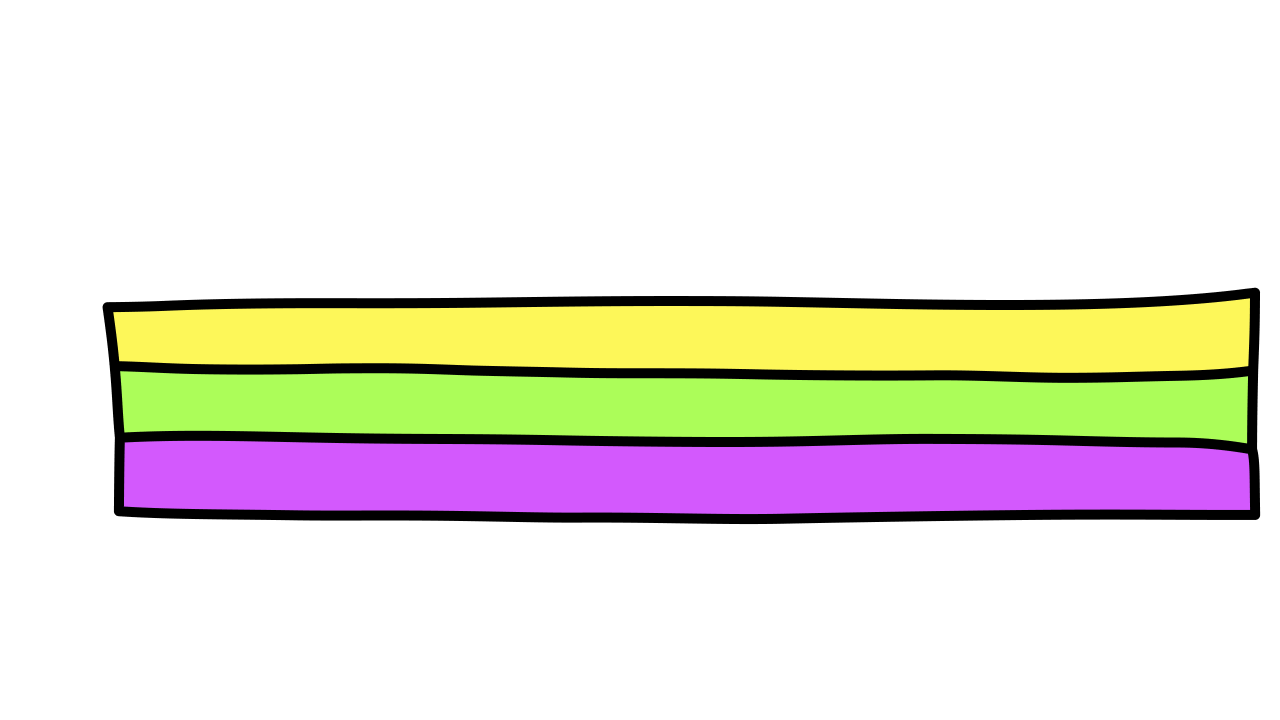
\includegraphics[width=.35\textwidth]{unFoldDescription1.png}\\
\end{tabular}
\caption{Un-Fold example.}
\label{unfoldeg}
\end{figure}\\\\
The full explanation of the un-doing proccess is explained in section ....

\subsection{Faults}
Like mentionned in section ~\ref{sub:fold} faults are the results of forces applied to the cross section and causing breaks. When a break appear, it divides a block into two others with one sliding on the other. This is the process we want to inverse by applying the correct opposit forces and sliding such as in Figure ~\ref{unfaulteg}

\begin{figure}[htb]
\centering
\begin{tabular}{@{}cc@{}}
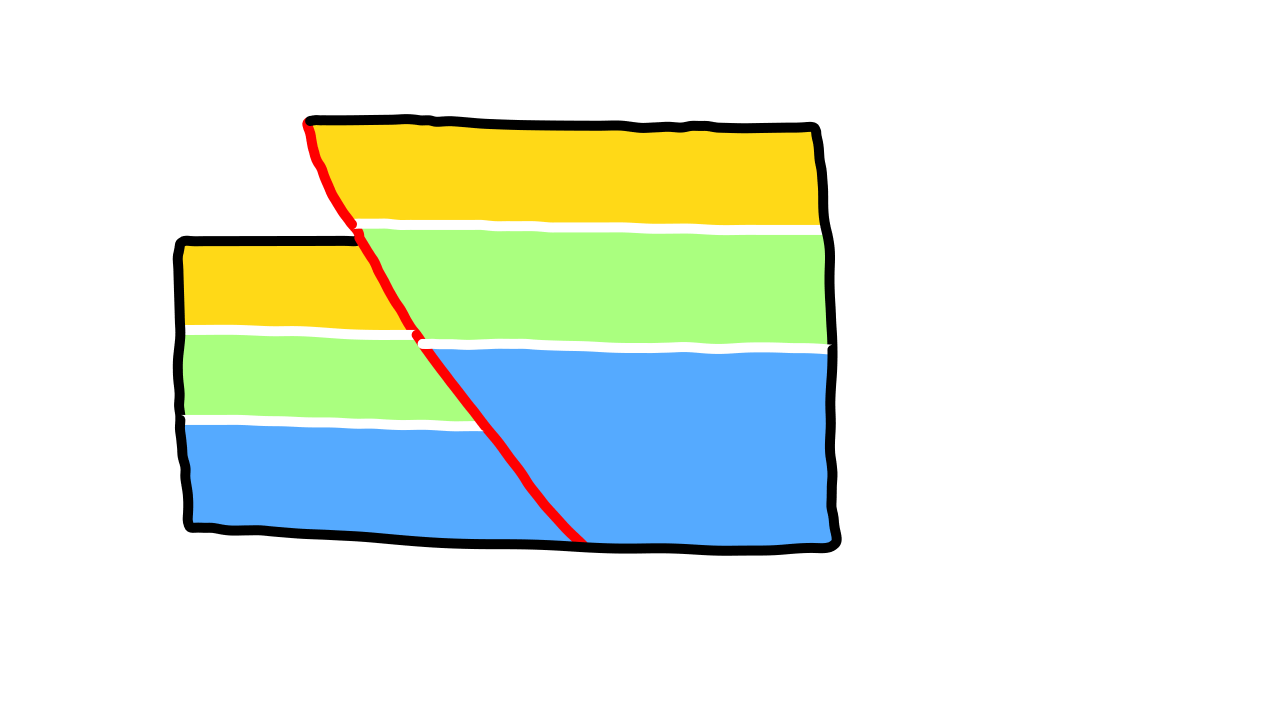
\includegraphics[width=.35\textwidth]{unFaultDescription0.png}&
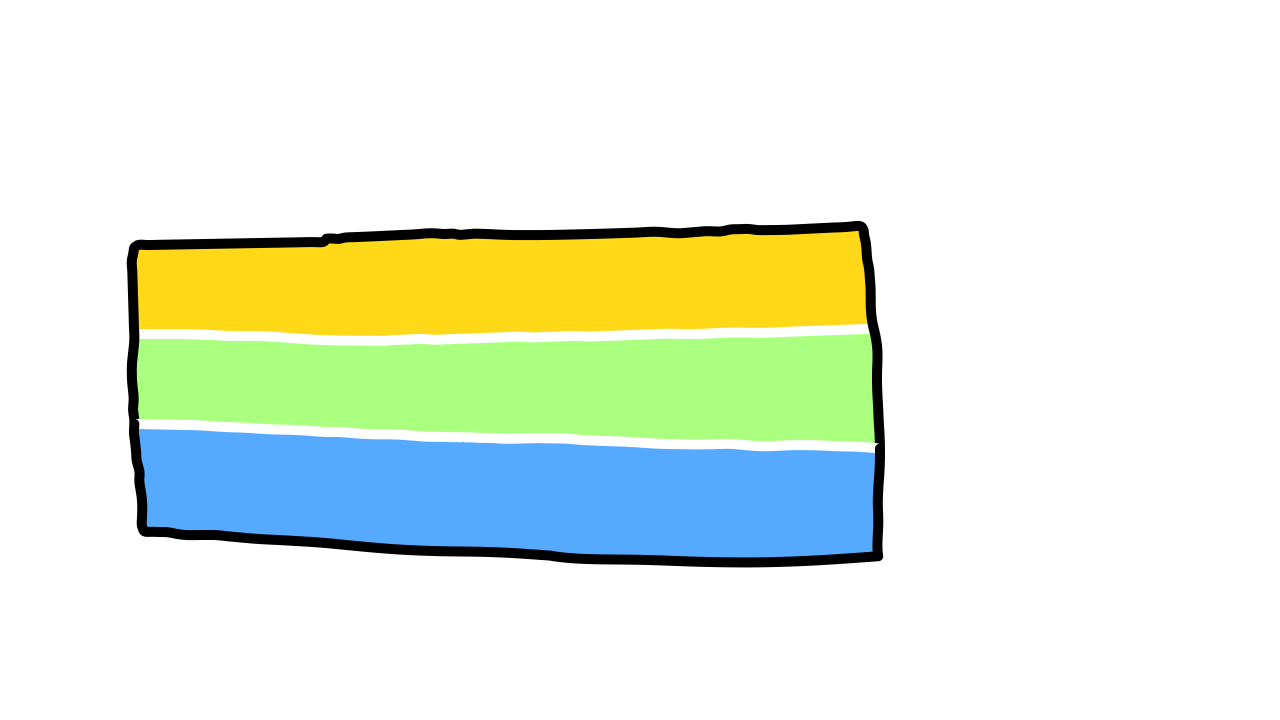
\includegraphics[width=.35\textwidth]{unFaultDescription1.png}\\
\end{tabular}
\caption{Un-Fault example.}
\label{unfaulteg}
\end{figure}\\\\
The full explanation of the un-doing proccess is explained in section ....

\section{Story Telling process}
\label{sub:storytel}
In order to offer an interactive process of creating plausible restoration scenarios, we proposed a story telling method using two graphs. One being the Story Tree which allows the user to choose a list of events to simulate at each node among a list of possible events to simulate. A node correspond to a cross section situation back in time while a branch corresponds to the choosen events' simulation. Then, starting from an arbitrary node, it becomes possible to go back in the tree and chose other events to un-do for exploring other scenarios.\\\\
The other graph we use in our process is the Event Graph which contains all the identified events we can detect at time $t = 0$, when loading the section, as well as their time dependency with each other. This graph is the base of our event proposition model for the Story Tree as it allow us to keep a time coherence in our restoration process. The Story Tree model is described in section ... and the Event Graph one in section ...
\section{Animation model}
Because the goal of this project was to provide an interactive method to build and visualise our different scenarios, we needed simulation times to be small, near real time.We propose an animation model which combines physically based and geometrically based methods. The main animation loop consist in using mass-spring systems mapped on our cross-section and apply a Implicit Euler Scheme on it. On the other hand we propose external operators simulating our un-doing events which use geometrical algorithms. The computation times are real time regardless the event we simulate. The full animation system is described in section ~\ref{ch:animationmodel}.\\\\
After simulating un-do events the user can evaluate his choice visually and choose his next action. However our animation model allow us to give the user some hints about the success rate using deformation energy (see section ~\ref{sec:generalanimation}).
%Indeed as we mentionned in section ... sedimentation always occur horizontally at the surface. Because the last event to undo will be sedimentation we can give the user a deformation rate of the spring which tells him to what extend the layer is horizontal . We can give this indication to the user each time we wants to do an un-sedimentation.
\section{Input Data Structure}
In our geological case we encounter many different topological configurations in the cross-sections. Indeed as we mentionned in our introduction ~\ref{ch:intro} cross sections are composed of sedimentary layers, fault and blocks. Each block contains part of superimposed layer which are called units and their side show discontinuities with its neighbouring block. Each layer is colored with a unique color representing the period it has deposited. Topologicaly speaking our cross-section is a convex graph composed of faces representing the units, which means that every face as at least one neighbour and there are no isolated group of faces. The discontinuities we find in the cross section are due to faults creation caused by extreme folding conditions. As a consequence we decided to use the VGC \cite{vgc} structure to encode our cross section as it can model all possible incidence relations between vertices, edges and faces in 2D sketches. We can notice than using such a structure allows us to extend our line of work in other field than geology.

\section{General WorkFlow}

Here we present the general workflow  of our methods which consists in five steps:\\\\

\indent 1) Event Graph generation by analysis of the input (chapter ...)\\
\indent 2) Story Tree recursive process of choosing events amoung a list of possible events to un-do\\
\indent 3) Animation of the list of choosen events \\
\indent 4) Either looping to the Story Tree process 2) or stoping the process and save the animation in a VAC XML file\cite{vac} (chapter ...)\\
\indent 5) Reading the VAC in reverse to show the forward cross section history

In the rest of our thesis, we describe more preciselly each step of our method. We first detail our story telling model with a complete description of the Event Graph and Story Tree processes. Then we detail our animation model  which include a main animation loop and external animation operator dealing with un-do event simulation. Afterwards we present our method implementation. Then show our results and finally conclude about the potential and the future works of the method. 

\chapter{Story teling}

In this chapter we present our story telling process which consist in detecting and ranking geological events and propose, in a recursive process, to user to choose events to un-do until he reaches the desired restoration.
We will first present our Event Graph data structure which store and rank the detected events. Then we will describe our Story Tree data structure which includes the event proposition recursion.

\section{Event Graph Generation: Scheduling and ranking Events}

As the main goal of our method is to propose recursively events to un-do and simulate them, we need a mean to propose the right list of possible event at each step. This is done by our Event Graph structure which rank geological events regarding their time dependency with each other and their probability of occurence.

When loading the input cross section, we are able to identify events to undo and create time dependencies between them just by looking at tgeological and geometrical properties of the section. Indeed they are obvious time relations we can deduce just by looking at sediments' ages. For instance we can sort the un-sediment events by looking at them. The youngest sediment will be the first one the user will un-sediment and the oldest will be the last. It is also obvious that un-erode events of one material must occur before its un-sedimentation. 
We can go further try to build less obvious time dependencies which uses topological properties. This is the case of un-fault event time dependencies. By checking their topology, we can determine if there are units of adjacent blocks which are already stuck together. Indeed a fault always shifts a matching unit (of the same material) by a offset when it is in activity. Thus if we find already stuck units along the fault we can deduce that the fault stopped its activity before the sedimentation of those unit's materials. Figure ~\ref{faultstick} Shows an example of this situation:\\\\
%example
	\begin{figure}[H]
	\centering
	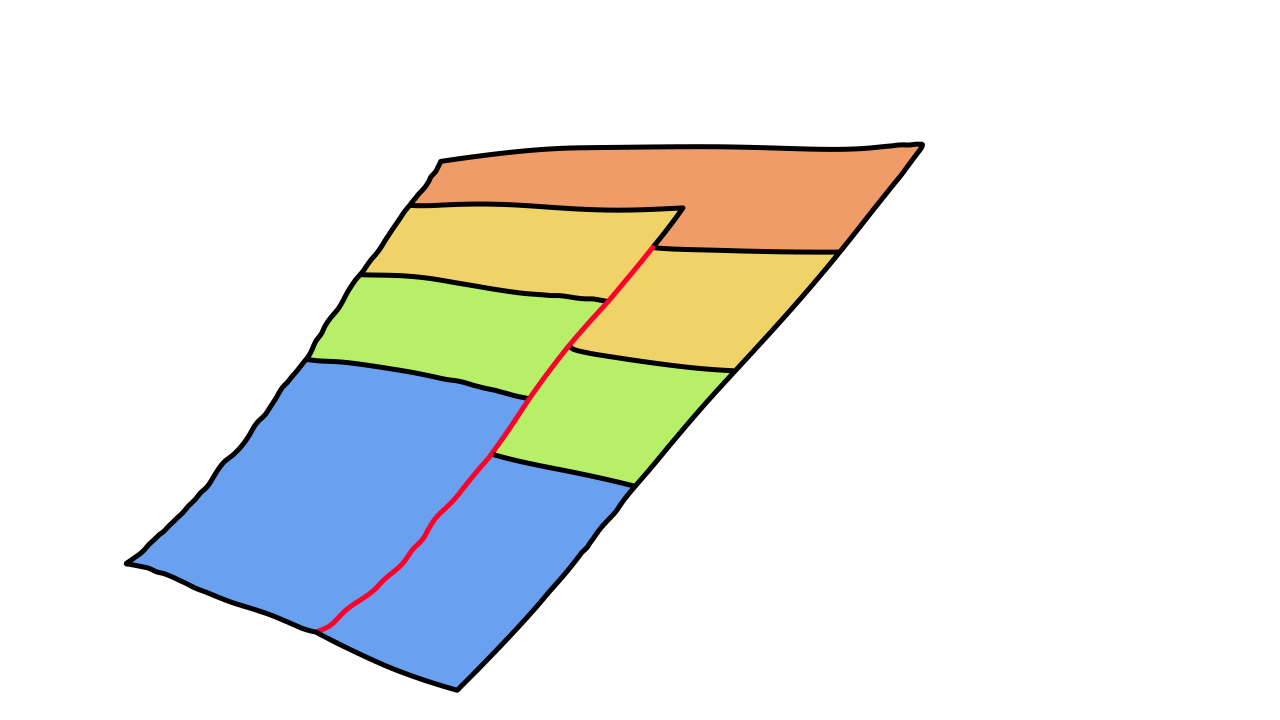
\includegraphics[scale=0.5]{unFaultSedDescription.png}
	\caption{Fault which ended before the sedimentation of the youngest orange layer. Here the orange layer is composed only of one unit (or two already stuck ones) whereas the others are composed of two non sticking units.}
	\label{faultstick}
	\end{figure}
	
After having build the time dependencies between events we store them in the Event Graph as follows:
one event will be stored as a node of the graph while a time depency will be stored as an oriented edge. An edge points to an other event which occured before (in the forward time way) the pointing event. If we take the example of two un-sediment events of one young material and one older than previous, the young un-sediment event will points towards the older un-sediment event like shown on Figure ~\ref{eventGraph} which is the event graph of Figure ~\ref{faultstick}:

	\begin{figure}[H]
	\centering
	\includegraphics[scale=0.5]{eventGraph.png}
	\caption{ Event Graph of Figure ~\ref{faultstick} which is composed of four un-sediment events and one un-fault event.}
	\label{eventGraph}
	\end{figure}

Thus the Event Graph contains possible un-doing events with time dependencies and will play the main role in the event propositon process in section .... However, as too many event propositions will come out this process (20 events to un-do at each step in the Chartreuse example), we decided to grant our Event Graph an additionnal way of ranking events; we will concider events' probability of occurence. In addition of containing an event, an Event Node will also contain an evaluation function which gives the probability of an event to occur at time $t$. This ranking will allow us to cut branches in the Story Tree and avoid unplausible scenarios exploration see section ...
.

Here are some example of evaluation function we used:

 - Un-fault (see section ...): We compute the side length of each of the two blocks' units which are in contact at the fault. The smaller the sum of the differences of each same material unit side length is the greater is the probability for the un-fault event to occur. It is justified by the fact that when a fault is closing it is done almost instantly with all the matching units facing each other\\\\
 
 - Un-eroding a concavity (see section ...): the wider the concavity is the greater the probability of occurrence is for this event. It is justified by the fact that keeping units having the same thickness on all their length is important to go back in time because at the restoration time they have the same thickness every where for the same material. Thus big eroded part must be the first ones to un-erode in order to assure the success of the simulation.\\\\

In the following section we will describe the Story Tree recursive process for proposing un-events which uses the Event Graph we build when loading the input drawing.

\section{Story Tree process: Proposing events and create scenarios} 

In this section we describe our event proposing recursion which will allow the user to build different restoration scenarios which is the hearth of our contribution.

This recursion process starts after building the Event Graph we just described and which contains the geological events to un-do with their time dependencies. The process works as follows: at each recursive step (time $t$) we propose a list of un-do events to the user provided by the Event Graph which select events not constrained by time dependencies at time $t$. Furthermore, as we mentionned in the previous section less palusible events will not be proposed and the system will encourage the user to un-do event with the largest probability first. This way we proceed to a branch and bound method for our scenario exploration. \\\\
In addition some events are not stored in the Event Graph and are only detectable at a given step $t$. For instance un-eroding concave parts (see section ... ) is only detectable at a given moment because concavities can appear and disappear while the whole terrain is deforming when un-doing other events. As a consequence, at each time step where an un-do event ends we have to detect this kind of event and propose it to the user. We will call this kind of event Dynamic event as they are only proposed at a given recursive step. In addition events such as un-Fold (see section ...) are not always detectable and must be provided user. That is why he has the opportunity to add its own Dynamic events when choosing among the list of possible events. Those events will be denominated as User Events.\\\\
To summerize, the list of proposed event at step $t$ is composed of events selected from the Event Grah, dynamic events only un-doable at this step $t$ and user events added bt the geologist. The final step for compelting our proposition list is to remove events which don't fulfill their starting precondition which is necessary to simulate them (see section ...).\\\\
Having this list of proposed events, the user can choose several events to un-doamong and simulate them. Afterwards he will wait for the simulation to end and will have three choices: loop to the recursive event proposing step and continue exploring one scenario, backtrack his action and explore new ones or end the process when obtaining the desired restoration scenario where there are no more events to undo.\\\\

This recursive process will be encoded in a Story Tree where each node contains the the list of event we can simulate at time $t$ and an edge represents the events simulated between two nodes. By encoding our process with this structure the user can explore as many restoration scenarios as he wants by following paths in the tree.

Figure shows an example of a Story Graph generated on the example of Figure ~\ref{strorygraph} :
%example story graph

\begin{figure}[htb]
\centering
\begin{tabular}{@{}cc@{}}
\includegraphics[width=.35\textwidth]{storyGraph.png}&
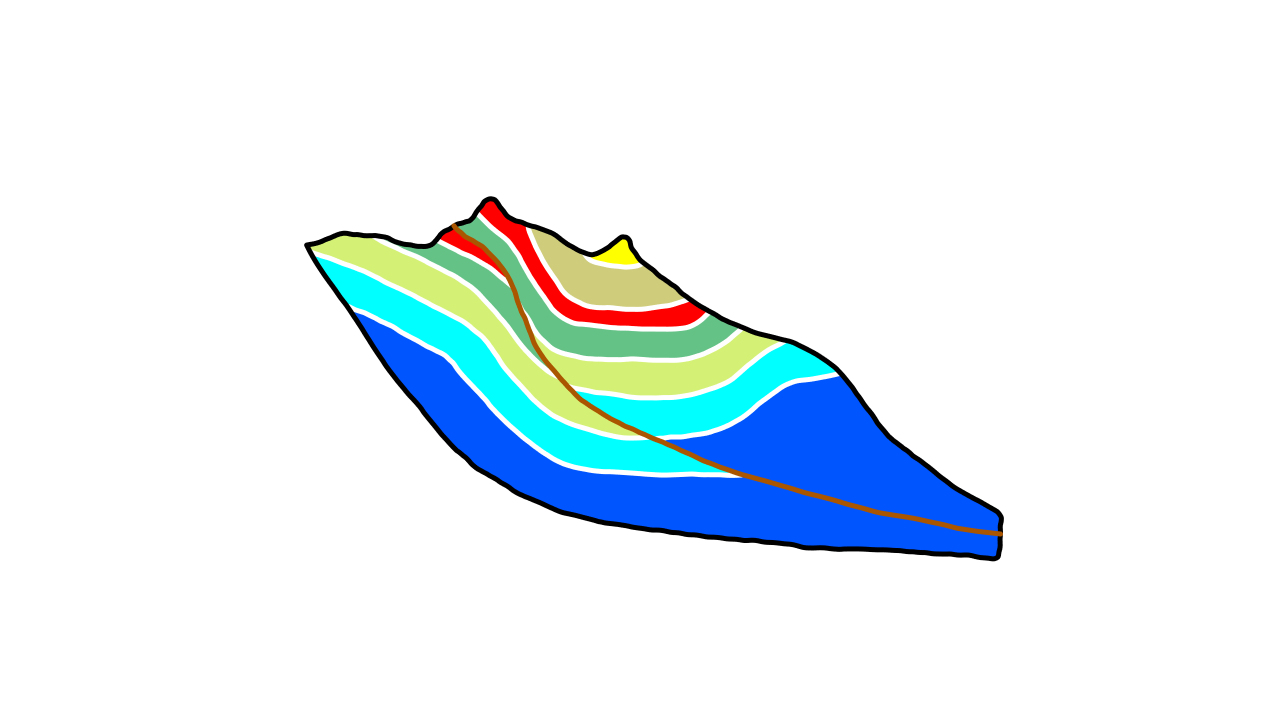
\includegraphics[width=.35\textwidth]{chartreusedroite.png}\\
\end{tabular}
\caption{Story Graph of a portion of Chartreuse cross section. Colored circles correspond to the un-sediment event of a given layer while rounded squares correspond to the only un-fault event present in this cross section}
\label{strorygraph}
\end{figure}\\\\

We presented our structure to creating interactively multiple restoration scenarios when several of them actually exist. In the next section we will present our animation model which will simulate the events we un-do during our recursive process.\\\\

\chapter{Animation Model}
In this chapter we will present our animation model which is composed of a main animation loop using mass spring system, deforming and moving our blocks and units, and of event simulation operators which apply additionnal operations in our section in order to un-do events.The output of our method we will a series of inbetween VGC encoded in a VAC which will be played on VPaint sofware \cite{vpaint} as it let the user choose the animation framerate.\\\\
\section{General animation loop}
\label{sec:generalanimation}
Here we will present our main animation method which is base of our cross section restoration simulation. 
The main idea of our method is to map a mass spring system on each block of the cross section and apply an implicit euler scheme solving the Newton's second law while possibly freezing the physic of several blocks at each time step regardless the undoing geological event. 
Our simulation is parametrized by information provided by the user (see section ...) such as deformation layer's deformation coefficient (Young Modulus) and friction coefficient (used in the Coulomb theory)

Like mentionned above the animation will be done by mapping a mass-spring system on each block.To be more accurate the systems are mapped on each units of each block. We proceed this way to take into account each unit orientation in the mapping as it is mapped according to unit's borders gradients. Considering that each unit is a rectangle that underwent some deformations the mapping will be done following the steps:	\\\\		
\indent	- First we have to put the masses both at the layer border but also inside it.\\\\
\indent	- We put the masses on the borders in an uniform way.\\\\
\indent	- We put the masses inside the unit: to do so we have two solutions:\\\\
\indent \indent	- Compute Hermite curve between each pair mass of the two level bounds and place particles uniformly on those curves.\\\\
\indent \indent	- Compute the intersections between the previous Hermite curves and the one coming from each pair mass of the two sides and place particles at those intersections.\\\\
	Even if the second solution might show better results that the first one we have chance that the curve comming from the sides might be not inside the layer due to big deformation making the layer non convex. \\With the first solution this problem is unlikely to occur because of the type of the deformations. In either case the Hermite curves be created using a mass pair and the gradient of the broder at each extremity as tangents. This way the layer will tend to transform back to a rectangle shape.\\\\
\indent	- Link particles with springs. \\\\We divide springs into 5 categories like described in \cite{cloth}: Vertical, Horizontal, DownShear, UpShear and Flexion. Adding flexion spring show better results in terms of shape preservation and breaking prevention. The resulting network looks like:\\
	
	\begin{figure}[H]
	\centering
	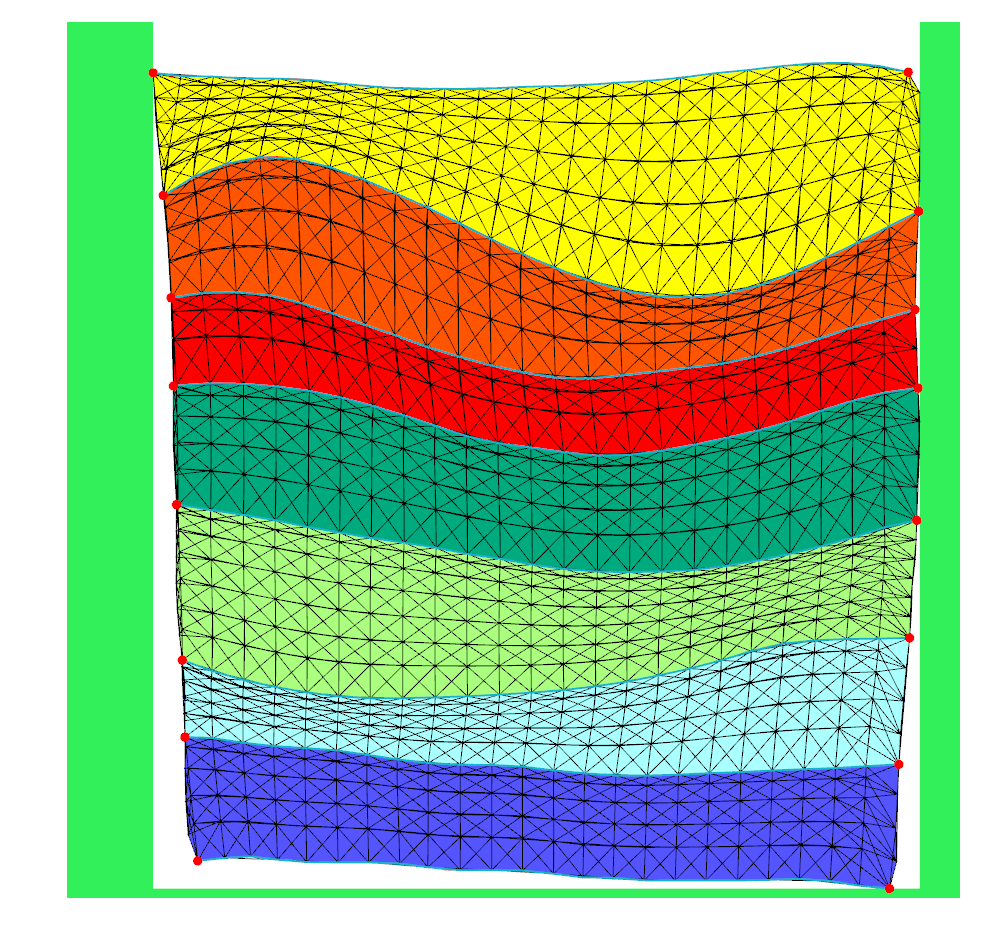
\includegraphics[scale=0.5]{springMapping.png}
	\caption{Mass-Spring Mapping on a block.}
	\end{figure}
	
	\indent	- In addition the stiffness of the springs which affect the way the unit deforms will be proportionnal to the unit material Young modulus. \\\\
\indent	- The springs we use will also have a torsion resistance in order to accentuate the shape change of the layer.\\\\
In terms of physical equations for a single mass spring system we use the implicit euler scheme and algorithm descibed in \cite{caltech}. We use this scheme instead of an explicit one because it is proven to be more stable with big time step ($dt = 0.02$).\\\\ 
Each particle has the same mass $m$ and possesses at step $n$:\\\\
\indent	- A position  $x_i^n$\\\\
\indent	- A speed $v_i^n$ \\\\\
\indent	- Applied forces $F_i^n$ (containing filtered, corrected and external forces).\\\\
At each time step we will solve the second Newton's law:\\

\begin{align}
	v_i^{n+1} &= v_i^n + F_i^{n+1} \frac{dt}{m}\\
	x_i^{n+1} &= x_i^n + v_i^{n+1} dt 
\end{align}

with:

\begin{equation}
F_i^{n+1} = - \sum\limits_{j|(i,j)\in Edges} k_{ij}(x_i - x_j) + k_{ij}l_{ij}^0\frac{(x_i - x_j)}{||(x_i - x_j)||}
\end{equation}


For each particle we want to integrate the above equations. The problem is that we don't know the forces at step $n + 1$ as we don't know the position of the particles at this step. That is why we use a first order approximation to solve the problem at step $n + 1$:

\begin{equation}
	F^{n+1} = F^n + \frac{\partial F}{\partial x}(x^{n+1} - x^n)
\end{equation}

\noindent Thus we need to compute $H =  \frac{\partial F}{\partial x}$ which is the Jacobian of $F$.\\\\
\noindent By using (1) and (4) we have the following result:
\begin{align*}
	(x^{n+1} - x^n) &= (v^n + (v^{n+1} - v^n))dt \\
	(v^{n+1} - v^n) &= (I - \frac{dt^2}{m}H)^{-1}(F^n + dt H v^n)\frac{dt}{m}
\end{align*}

We now have approximated our equations into a solvable system and we can notice that an additionnal force came from this approximation $dt H v^n$ . It is an implicit viscosity that takes into account the movement of the neighbouring particles.
Consequently we have for each particle $i$ a new force:

\begin{equation}
\tilde{F_i} = k dt \sum\limits_{j|(i,j)\in Edges}(v_j - v_i)
\end{equation}


The last thing to compute is $H$. Like in \cite{caltech} we will approximate $H$ by just integrating the linear part of the elastic force which is equal to:

\begin{equation}
F_{(i,j)} = -k_{ij}(x_i - x_j) + k_{ij}l_{ij}^0\frac{(x_i - x_j)}{||(x_i - x_j)||}
\end{equation}

If $H$ represents only the Jacobian of $F = -k_{ij}(x_i - x_j)$ it has the form:\\
\begin{center}
$
\left\{
\begin{array}{ll}
H_{ij} &= k_{ij} if i \neq j \\
H_{ii} &= -\sum\limits_{j \neq i}k_{ij}
\end{array}
\right.
$
\end{center}

Integrating only the linear part implies that we will have some error at the end of the integration. However we can notice that the non linear part $k_{ij}l_{ij}^0\frac{(x_i - x_j)}{||(x_i - x_j)||}$ has a constant magnitude during the simulation between two steps, so this force just implies a rotation that we will compensiate with another force. Thus we will correct the angular momentum $\delta T$ introduced by this method by adding correcting forces:
\begin{align*}
\delta T &= \sum\limits_{i=1}^n (x_G - x_i)\wedge F_i^{filtered} \\
F_i^{corrected} &= (x_G - x_i)\wedge \delta T dt
\end{align*}

with:
\begin{equation}
F_i^{filtered} = \sum\limits_{i=1}^n F_{ji}W_{ij}
\end{equation}

However in our case the equilibrum length of the springs will change over time creating an error in the angular momentum but we will try compensating this with torsion forces.\\\\

Finally we add torsion forces as external forces (along with gravity) because it is a non linear force and we can't integrate it:

\begin{equation}
F_{ij}^{torsion} = -k_{torsion}\Delta \theta \vec{n}
\end{equation}

with $\Delta \theta$ being the angle between a unit vector depending on the spring type (Vertical, Horizontal, DownShear or UpShear) and the vector $x_i - x_j$. $\vec{n}$ is the normal vector to $x_i - x_j$ pointing toward the unit vector.\\\\

Finally we can add a optionnal inverse dynamic step at the end of the scheme loop which consist in correcting spring angles which make quads or triangles to be inverted causing face self intersection. Actually the torsion we already apply helps to prevent for having this case it is not given. Consequently here we impose that $\theta < \frac{\pi}{2}$ 

Computing a mass spring system can take some time (few seconds for big systems) and can be noticable especially during block fusion but that is not a problem because the goal of the project is to record at each time step the result of our simulation as an inbetween VAC which can be played fluently.\\\\

\section{Geological Events Simulation}
In order to simulate an event, it has to fulfill preconditions which are required for the simulation and to ensure geological consistancy. Then when an event is simulated it has also post conditions to fulfill in order to transform the cross section into the state it was before this event. With this convention, simulating an event is equivalent into inbetweening the section from the precondition to the postcondition state. Furthermore all the simulated events evolve in the same time line having a duration which can be set by the user depending on the event.\\\\
\chapter{Dealing With Discrete Geological Events}\\

As we mentionned earlier, geologists are usually able to restore the history of cross sections by using several geometrical and simulation tools. However they only get one sequence leading to the final state of the section which represents its the state before any techtonic movement. Here we are interested in what happened between today's section state and the restoration. Indeed most of the time, when restoring sections; there are several scenarios that lead the initial state to the restoration, that is why geolists often question others' hypothesis. This is exactly one of the main thread of this project. We want to explore the most plausibles scenarios and see the resulting animation of exploration.\\\\
To do so we will propose to the user to undo geological events at each time step. We can count already four events we want to undo : faults, erosion, sedimentation and  folding. Those events will be automatically detected and resorbed most of the time. It is possible to detect automatically faults, erosion and sedimentation but folding is something not present in the drawing, the applied forces are not shown. Therefore the user has to provide the un-folding even, meaning he has to choose when and how we want to apply it.\\\\ 

In order to encode our events in a intuitive manner we will use a story tree. However given the cross section we must determine the possible events to undo but also their time dependency with each other. For instance we know that the last event we will undo will be a sedimentation , that is why this un-sediment event must come after un-erode or un-fold events if this kind of event occured. In order to take into account this time dependency between events we will use an Event Graph to encode it. On the other hand, the story tree will be stored within a Story Graph which will be build thanks to the Event Graph and progressively expanded by the user.\\\\

The Story graph represents the different event sequences we can run the simulation on. A node represents the list of event we can simulate at time $t$ and an edge represents the events simulated between two nodes. The Event Graph is used in the creation of this Story Graph be cause it will be taken into account when proposing at time $t$ the list of possible event to simulate. As a result user will explore this graph as a tree and will be able to see the animation of as many scenarios as he wants to see.\\\\

Figure ... shows an example of Story Graph generated on a simple example:
%example story graph


Having a structure to create and come back on scenarios, we have to simulate the chosen events. To do so we have to set up the event structure which will allow the event to begin, being simulated and to end.\\\\

In order to simulate an event, it has to fulfill preconditions which are required for the simulation and to ensure geological consistancy. Then when an event is simulated it has also post conditions to fulfill in order to transform the cross section into the state it was before this event. With this convention, simulating an event is equivalent into inbetweening the section from the precondition to the postcondition state. Furthermore all the simulated events evolve in the same time line having a duration which can be set by the user depending on the event.\\\\

During this thesis we identified 4 events we could simulate with our given input data: un-erode, un-sediment, un-fault and un-fold. Each event has a very specific way to be simulated using the mass-spring model we introduced as its base.\\\\

Here we presents the way of simulating those events:

\section{Un-Sediment}

Un-sedimenting a layer consist in removing sediment progressively when the upper bound of the layer is perfectly horizontal as it is an unbreakable rule in geology.\\\\

In a sequence we will simulate the layer's thickness shrinking like:
%Dessin
\begin{figure}[h]
    \begin{minipage}[c]{.50\linewidth}
        \centering
        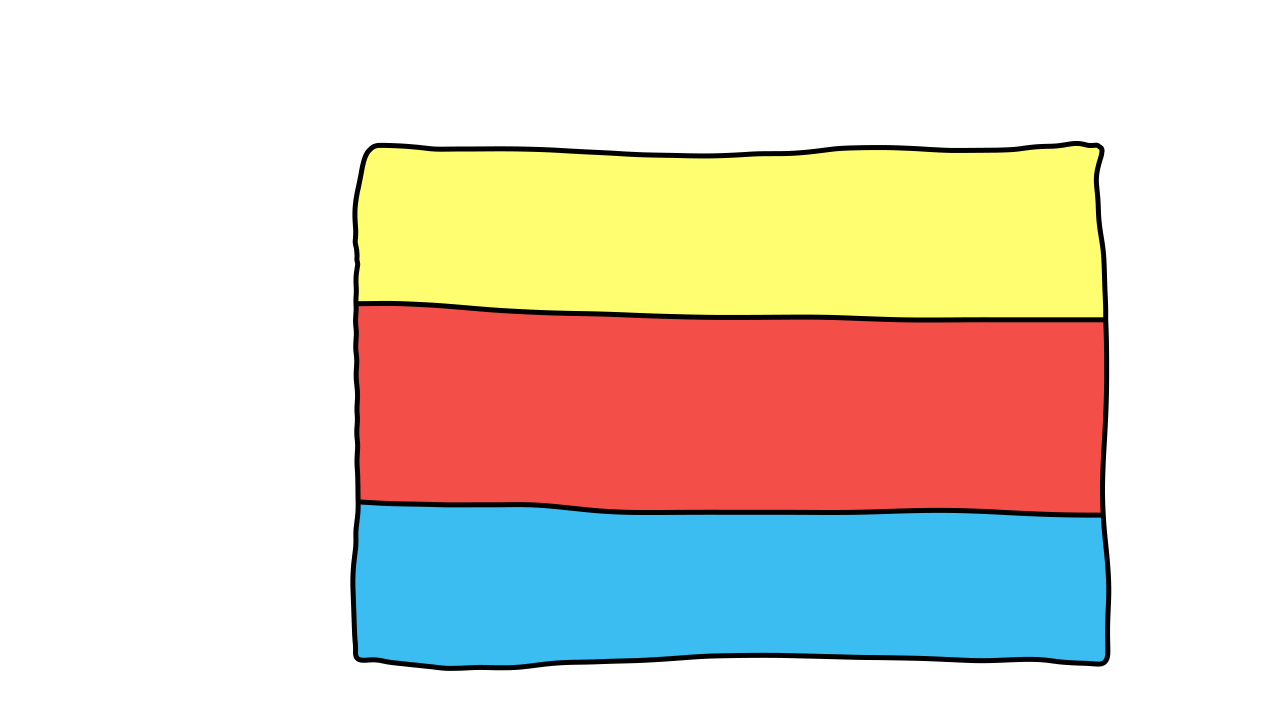
\includegraphics[scale=0.2]{unSedimentDescription0.png}
	\caption{Un-Sediment one layer example. Starting Configuration}
    \end{minipage}
    \hfill%
    \begin{minipage}[c]{.50\linewidth}
        \centering
        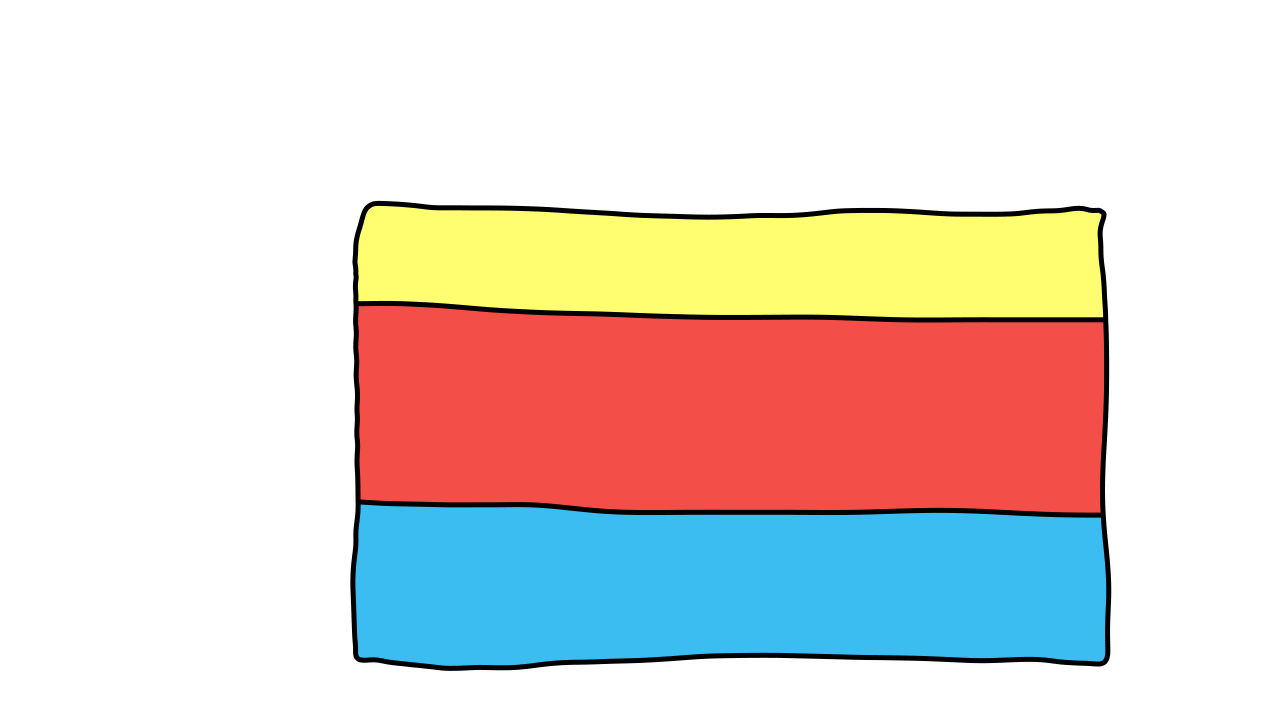
\includegraphics[scale=0.2]{unSedimentDescription1.png}
	\caption{Un-Sediment one layer example. Middle Configuration}
    \end{minipage}
     \hfill%
    \begin{minipage}[c]{.50\linewidth}
        \centering
        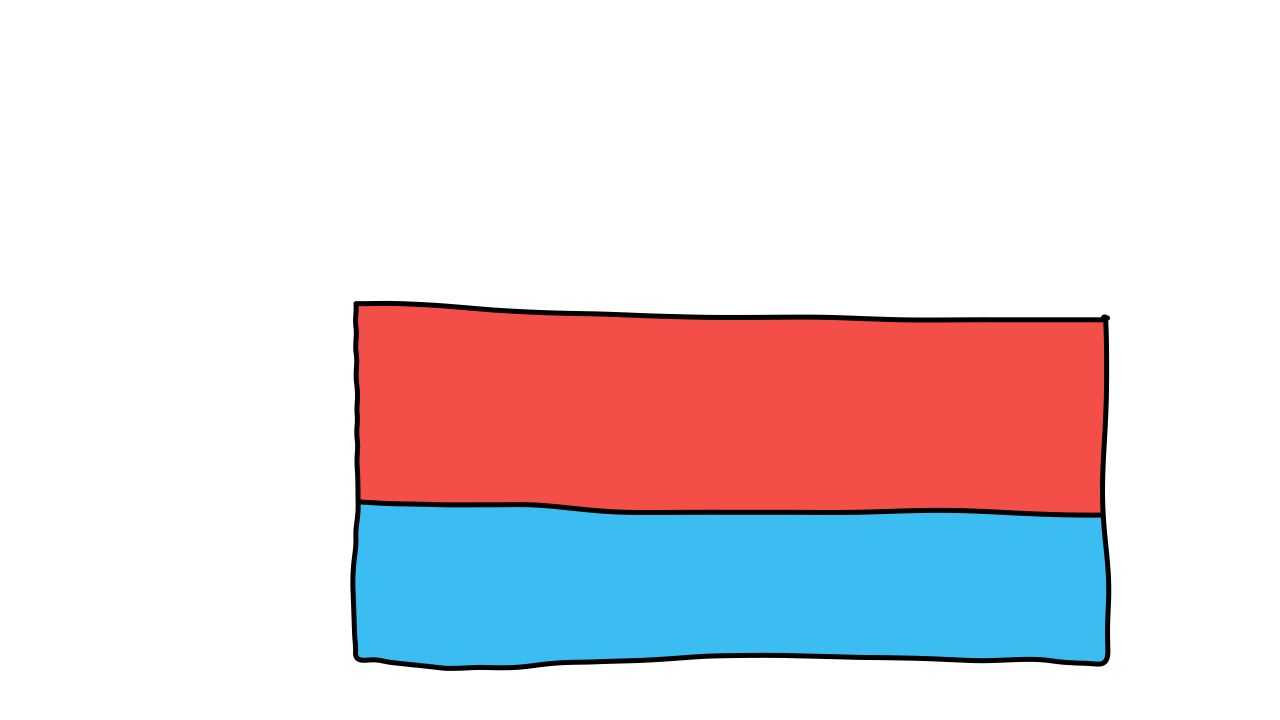
\includegraphics[scale=0.2]{unSedimentDescription2.png}
	\caption{Un-Sediment one layer example. Ending Configuration}
    \end{minipage}
\end{figure}\\
\textbf{Precondition:} the layer's upper bound must be horizontal and the layer must be the youngest in the section.\\\\
\textbf{Simulation:} we progressively decrease the equilibrium length of vertical springs until it reaches $0$ for all the vertical springs when the event end.\\\\
\textbf{Duration:} given by material's age we want to un-sediment.\\\\
\textbf{Postcondition:} the layer must have desappeared letting a new layer to be the youngest 
in the section.\\\\
\textbf{Postcomputation:} regenerate the mass-spring system of the containing block at the end of the event.\\\\

\section{Un-Erode}

In the cross section the erosion impact can be noticed by thickness variation in the same layer. However, it can have different effects topologicaly speaking depending on where it is applied. Here we will distinguish three different categories of erosion because of their topological and geometrical effects.\\\\

\subsection{Un-Erode block side}

Here we are interested in the erosion that occured at the side of the blocks which creates concavites and reduce the thickness of layers at some places. Here we will try to fill the concavities we can detect if they appear to have been created by an erosion process such as:
%dessin
\begin{figure}[h]
    \begin{minipage}[c]{.46\linewidth}
        \centering
        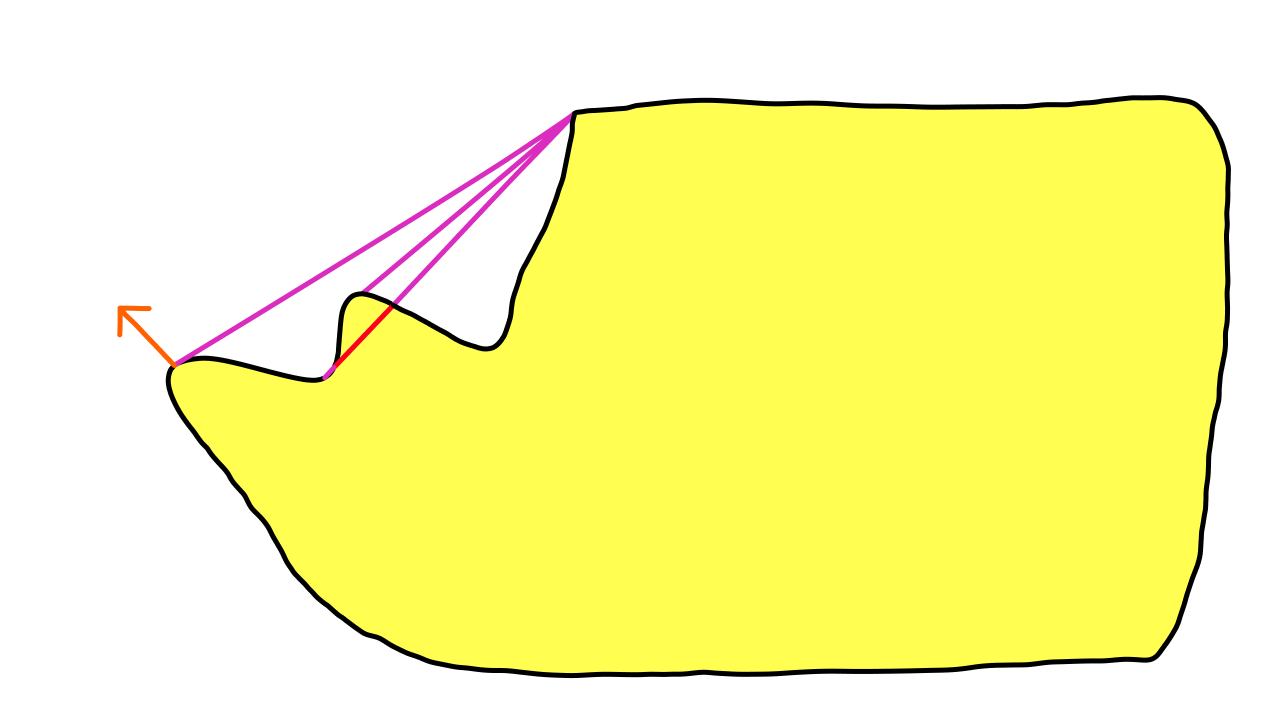
\includegraphics[scale=0.2]{unErodeSideDescription0.png}
	\caption{Un-Erode block side example. Starting Configuration}
    \end{minipage}
    \hfill%
    \begin{minipage}[c]{.46\linewidth}
        \centering
        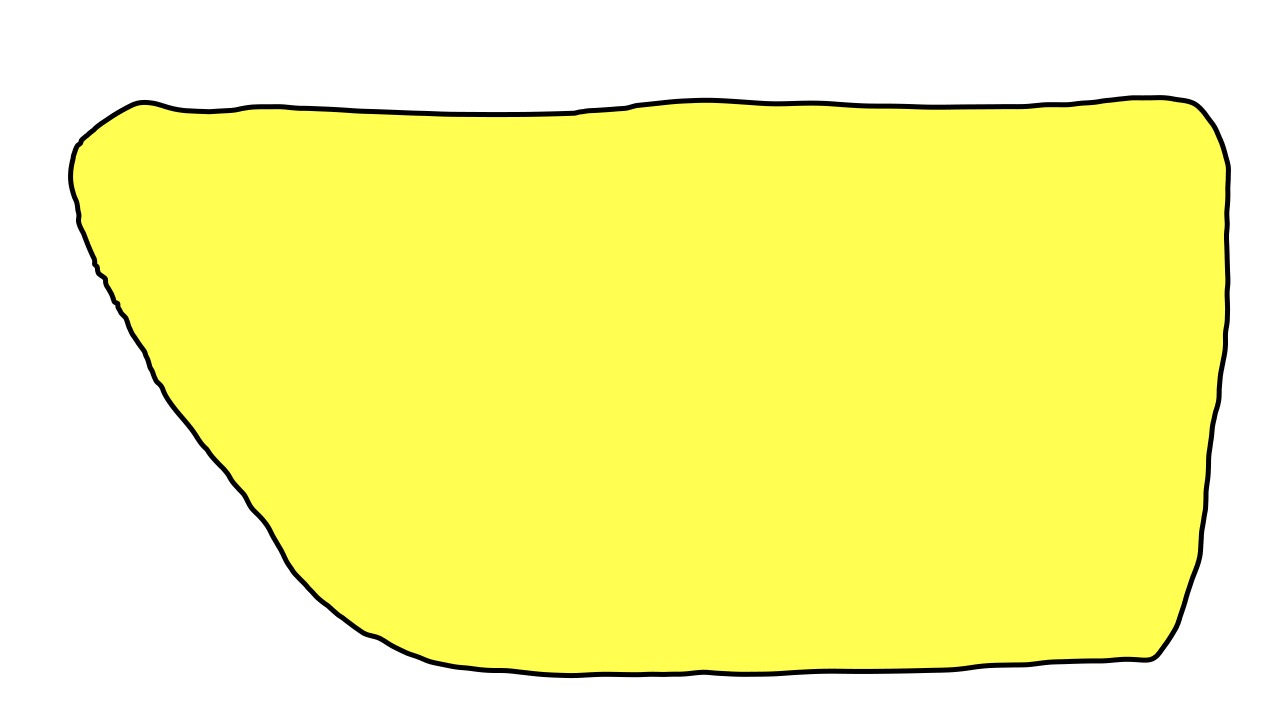
\includegraphics[scale=0.2]{unErodeSideDescription1.png}
	\caption{Un-Erode block side example. Ending Configuration}
    \end{minipage}
\end{figure}\\
This event is applicable to any surface module of the cross section.\\\\
\textbf{Precondition:} A concavity must be detected in the unit's sides. Here we are not interested in detecting all the concavities in the sides because some of them might have been caused by other events than erosion such as folding. Moreover we are interested in concavities which are between the upper corners of the units and its side. To be more precise we will fill an area between a upper side corner and the farthest side particle where there is a concavity in between. Progressively starting by the upper masses of the side and going down, we will look at the segment between the upper corner of the side and the considered particle. If the segment do not intersect the unit itself, then it is considered as a concavity. The final segment which we are interested in is the concavity segement between the corner and the farthest particle on the side. We store this particle and if it is different from the particle right after the corner then it means that there is a concavity to fill and the precondition is fulfilled.\\\\
\textbf{Simulation:}  Starting from this found farthest particle, we will compute the normal att his point and create a new mass following the line beginning at the found particle and directed by the normal. The new mass will be created at the point of same high than the upper corner in the normal line. This point will be the new corner of the unit and expand it as the new side will be projected toward the computed normal line.\\\\
\textbf{Duration:} given by the user.\\\\
\textbf{Postcondition:} the side that has been un-eroded must not intersect other units.\\\\
\textbf{Postcomputation:} regenerate the mass-spring system of the containing block at the end of the event.\\\\

\subsection{Un-Erode surface upper bounds}

Having treated the case of side erosion, we want also to un-do erosion that affected the upper surface of layers. Here concavities are not the only target we want to focus on. In this case erosion can easely let the surface being convex, so we will try to detect zones where the thickness of the layer decreased. Therefore we will look for zones in the upper bound where the curvature suddenly changed.\\\\
%dessin
\begin{figure}[h]
    \begin{minipage}[c]{.46\linewidth}
        \centering
        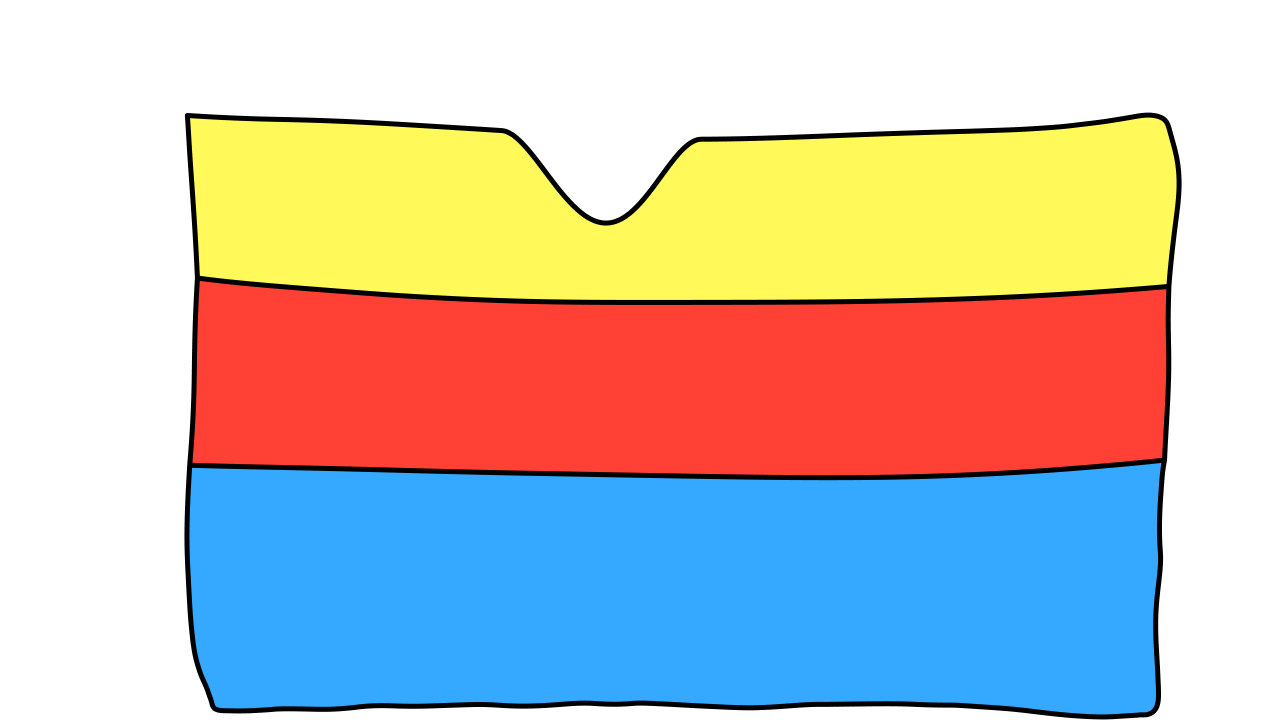
\includegraphics[scale=0.2]{unErodeUpDescription0.png}
	\caption{Un-Erode upper bound concavity example. Starting Configuration}
    \end{minipage}
    \hfill%
    \begin{minipage}[c]{.46\linewidth}
        \centering
        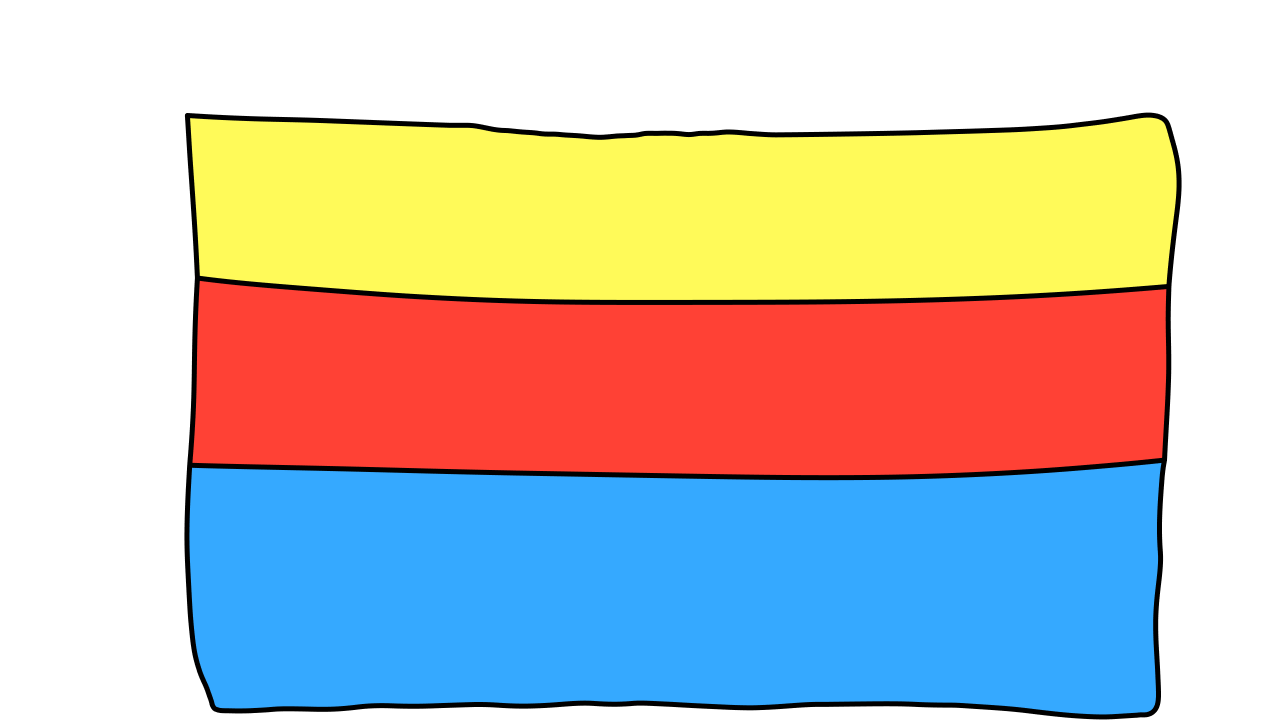
\includegraphics[scale=0.2]{unErodeUpDescription1.png}
	\caption{Un-Erode upper bound concavity example. Ending Configuration}
    \end{minipage}
\end{figure}\\
\begin{figure}[h]
    \begin{minipage}[c]{.46\linewidth}
        \centering
        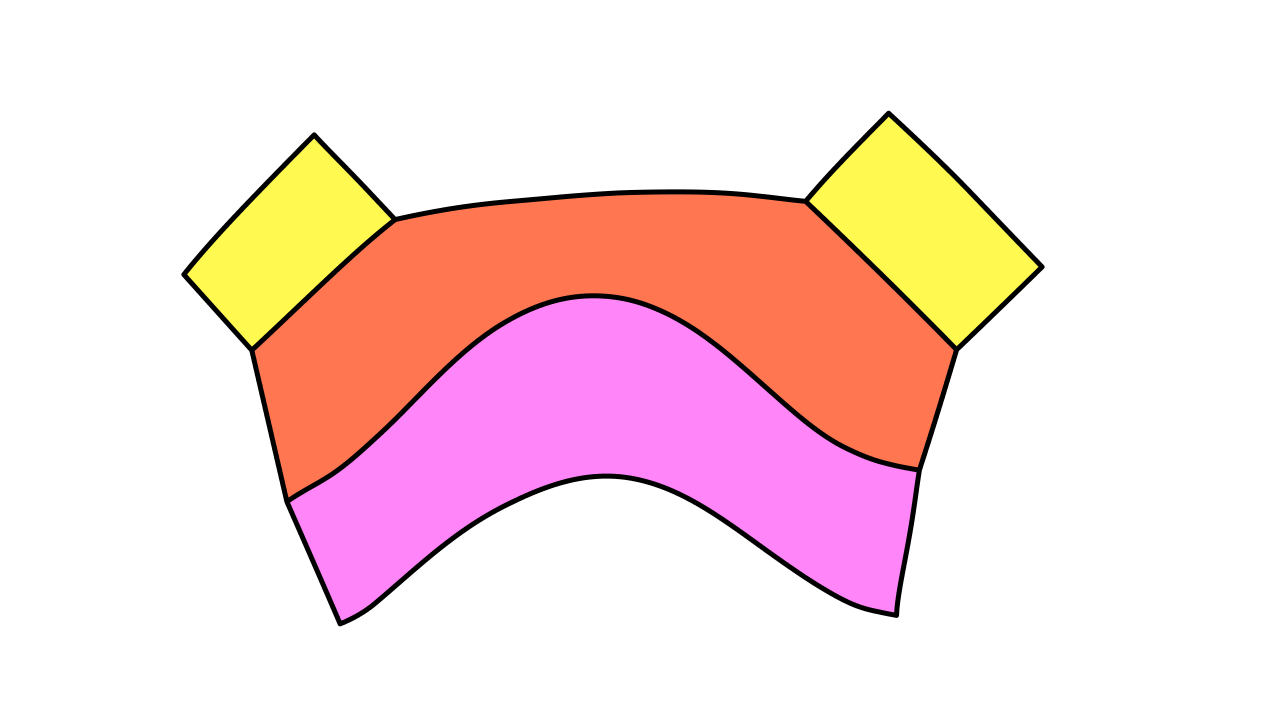
\includegraphics[scale=0.2]{unErodeConvexDescription0.png}
	\caption{Un-Erode upper bound in a hole example. Starting Configuration}
    \end{minipage}
    \hfill%
    \begin{minipage}[c]{.46\linewidth}
        \centering
        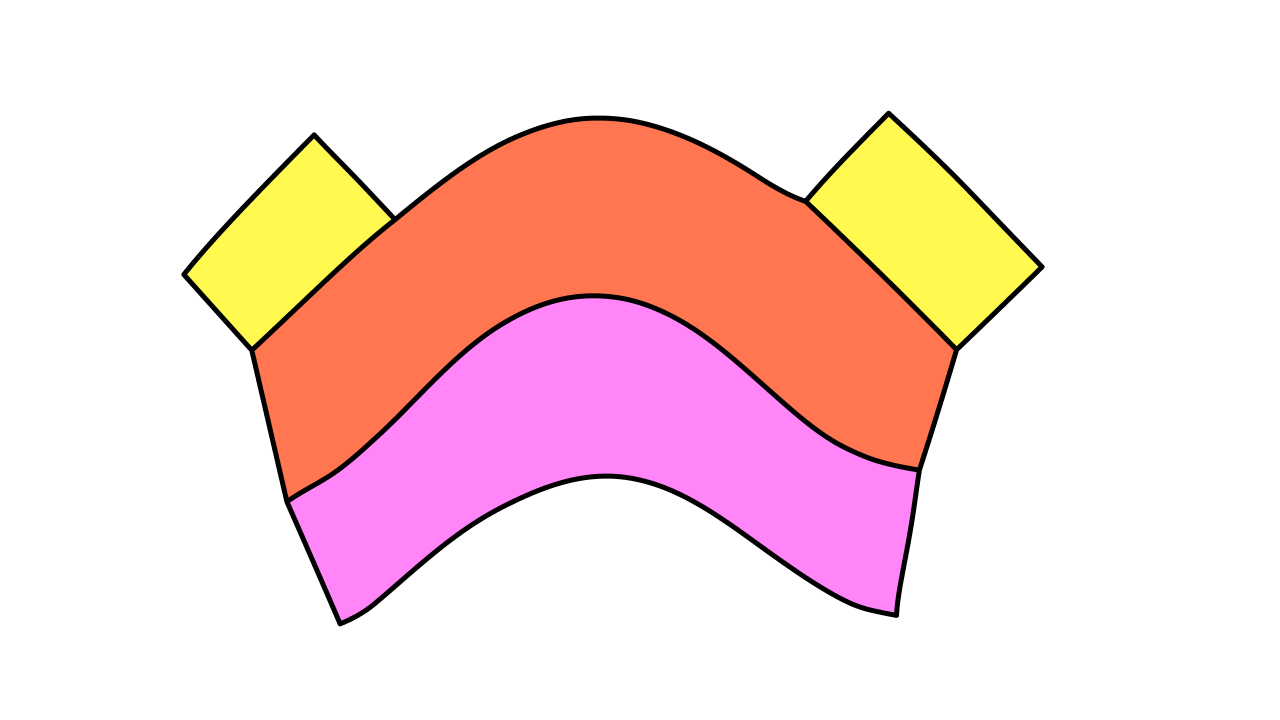
\includegraphics[scale=0.2]{unErodeConvexDescription1.png}
	\caption{Un-Erode upper bound in a hole example. Ending Configuration}
    \end{minipage}
\end{figure}\\
\textbf{Precondition:} the upper bound must be at the surface and must have either a concavity or a changing curvature at some point. To detect convaties this time we use mathematical properties of the upper bound curve because we don't want to miss one as any concavity can be a product of erosion in this case. Therefore we look at the upper bound as being a discretized parametric curve $(x(t),y(t))$ and we search for concavities. To do so we will compute the speed vector $(x'(t),y'(t))$ and the acceleration vector $(x''(t),y''(t))$ and look at the sign of $det(v(t),a(t))$. If it is negative it means that the curve is concave. Thus we search for every concave areas which are intervals $[t_0,t_1]$ where the the curve is concave. We can also check if the curve has a big change in its curvature and if this change doesn't create a concavity. This is likely to happen  in holes which dug through several layers. Here the eroded part of the surface upper bound is likely to be eroded even being convex. Here the change in curvature might be noticable and we propose to the user to un-erode those units when we detect such a unit configuration. As a consequence whenever we detec a surface bound in a hole which divided at least one unit into two we propose the un-erode event for a part the surface curve in an interval $[t_0,t_1]$ just like before.\\\\
\textbf{Simulation:} In both cases we will use Hermite curve to fill the lacking matter. We will use them with the following coefficients $I(t_0), I(t_1)$ which are the points at the beginning and the end of the eroded curve and $I(t_0) - I(t_0 - 1), I(t_1) - I(t_1 + 1)$  as tangent respectively at point $I(t_0)$ and point $I(t_1)$. Then we deform the current curve making it matching the computed Hermite curve. By proceeding this way we will fill abnormalities in the layers following the trajectory the curve should have if we un-erode it.\\\\
\textbf{Postcondition:} the abnormalities must have been filled.\\\\
\textbf{Postcomputation:} regenerate the mass-spring system of the containing block at the end of the event.\\\\

\subsection{Un-Erode two facing units of the same Material}

Here we are interested in the case where erosion happened in the middle of a layer, making a hole a dividing it into several units. We can note that this can happen for units which are in the same block but also for units in neighbouring blocks. Here we will merge the two divided unit by adding an interpolated part bewteen them.\\\\
%drawing
\begin{figure}[h]
    \begin{minipage}[c]{.46\linewidth}
        \centering
        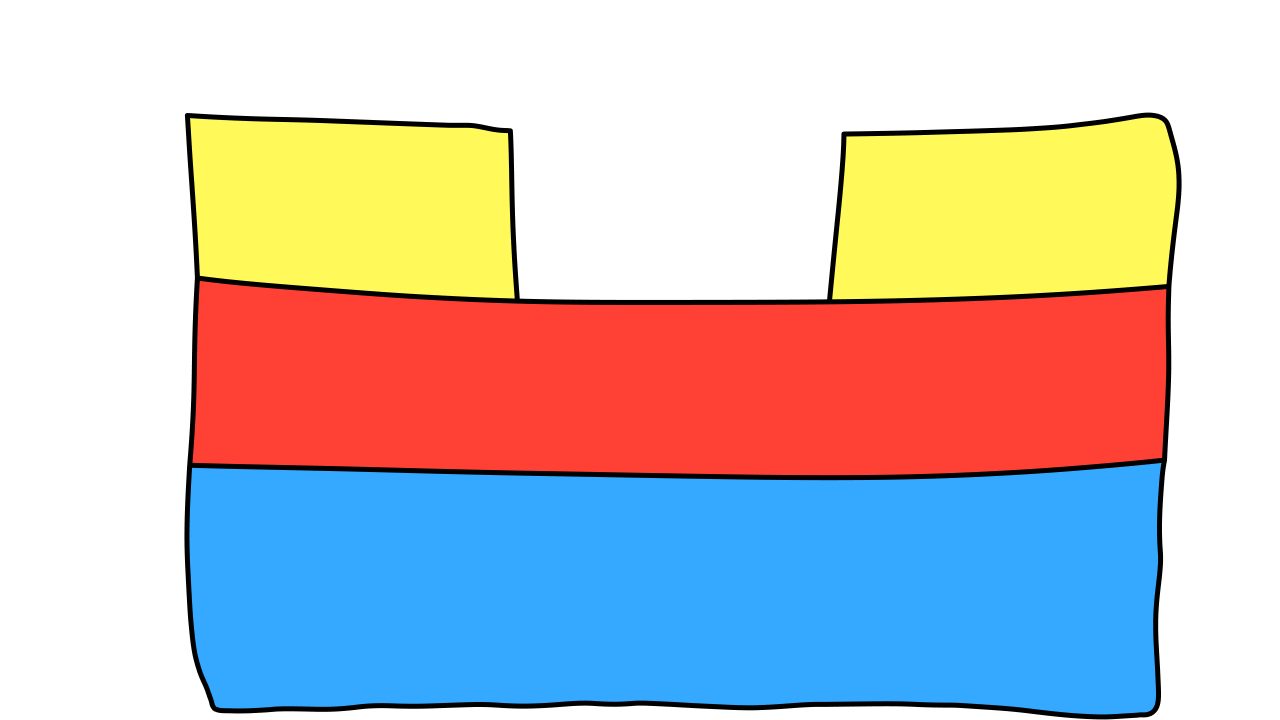
\includegraphics[scale=0.2]{unErodeTwoLayersDescription0.png}
	\caption{Un-Erode two facing units of the same Material in the same block example. Starting Configuration}
    \end{minipage}
    \hfill%
    \begin{minipage}[c]{.46\linewidth}
        \centering
        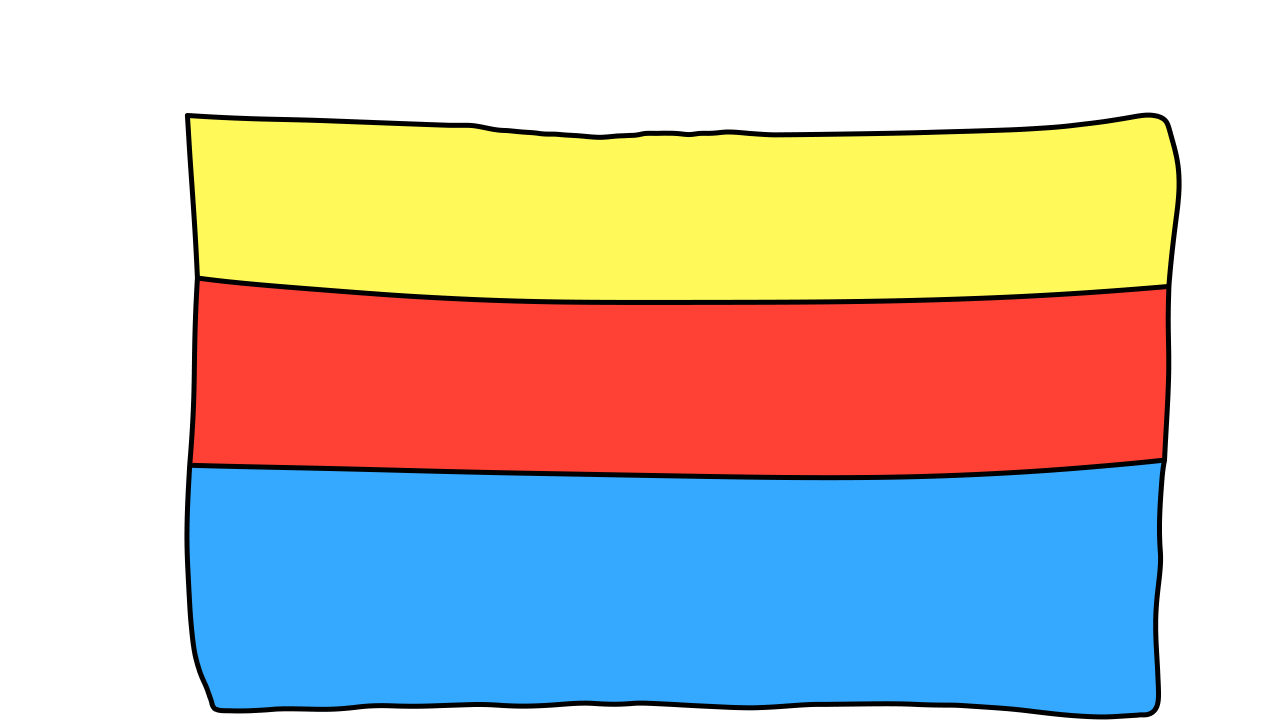
\includegraphics[scale=0.2]{unErodeTwoLayersDescription1.png}
	\caption{Un-Erode two facing units of the same Material in the same block example. Ending Configuration}
    \end{minipage}
\end{figure}\\
\textbf{Precondition:} the two units must face each other in all cases and not in contact in a fault if there are on different blocks. It is obvious that they should be of the same material. Finally if there are in a hole that divided older layers we cannot un-do this erosion before un-doing the erosion of those layers.\\\\
\textbf{Simulation:} Here we will use Hermite curve again for the same reason of preserving the curvature continuity. If we are in the case of units between blocks, we will use an Hermite curve joining the two upper bounds and one joining the two bottom bounds and fill the zone delimited by these two curves. If we are in the case of two units in the same block we only need to interporlate the upper bound as the bottom bound already exist.\\\\
\textbf{Postcondition:} the two units must have merged into a new one.\\\\
\textbf{Postcomputation:} regenerate the mass-spring system of the containing block at the end of the event.\\\\
\subsection{Un-Erode special case}

Finally we identified a last case of erosion which corresponds to the following configuration:\\\\
\begin{figure}[H]
	\centering
	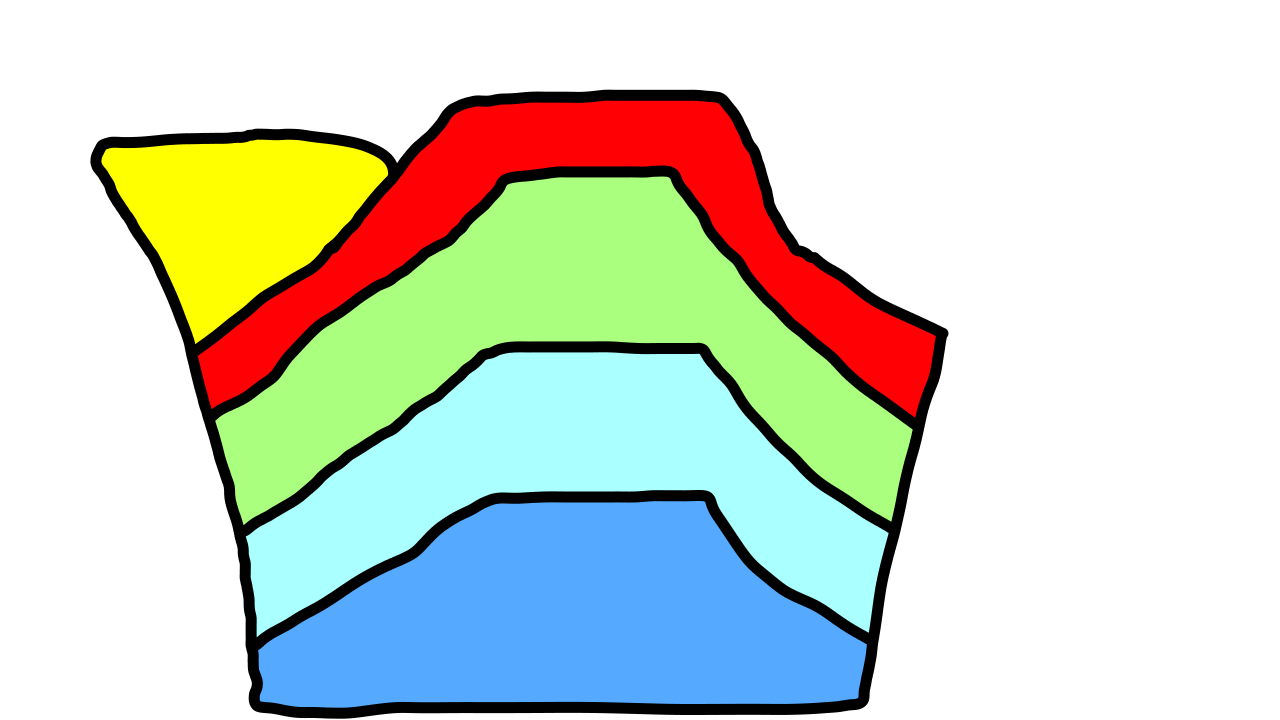
\includegraphics[scale=0.3]{unErodeSpecial.png}
	\caption{Un-erode special case}
\end{figure}
Here we can wonder if the yellow unit has been eroded.  It seems that there is lacking matter on the red unit and we want to add yellow sediment fill the surface part of this unit. However geologically speaking here we observe that the units are highly deformed and so the lacking part might not be one and the yellow sediment has only deposited in the left side because of relief shape. In the case we want to un-erode  the yellow unit we have add enough matter to fill all the red unit surface.\\\\
\textbf{Precondition:} the concerned unit must have free surface upper bound of the unit just under him.\\\\
\textbf{Simulation:} Here we just extend the concerned unit until the end of the free surface while increasing its thickness if it is necessary for filling the lacking part.\\\\
\textbf{PostCondition:} All the free surface bound must have been filled by the concerned unit sediment.\\\\
\textbf{Postcomputation:} regenerate the mass-spring system of the containing block at the end of the event.\\\\

\section{Un-Fold}

Un-Folding basically means applying forces on blocks, units or particles of the section. Theses forces can be applied in any manner such as uniformly or linearly. It is a event which is most of the time added by the user but plays also a major role in the un-fault event.\\\\
%dessin
\begin{figure}[h]
    \begin{minipage}[c]{.46\linewidth}
        \centering
        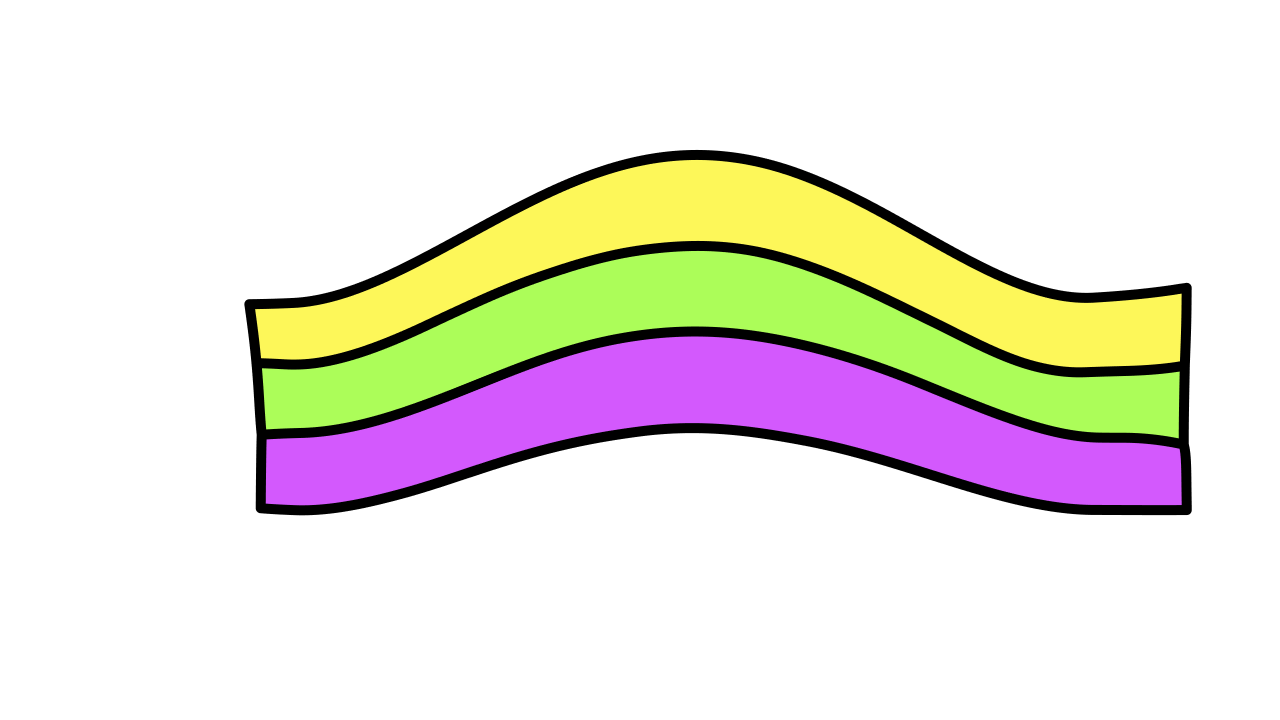
\includegraphics[scale=0.2]{unFoldDescription0.png}
	\caption{Un-Fold example. Starting Configuration}
    \end{minipage}
    \hfill%
    \begin{minipage}[c]{.46\linewidth}
        \centering
        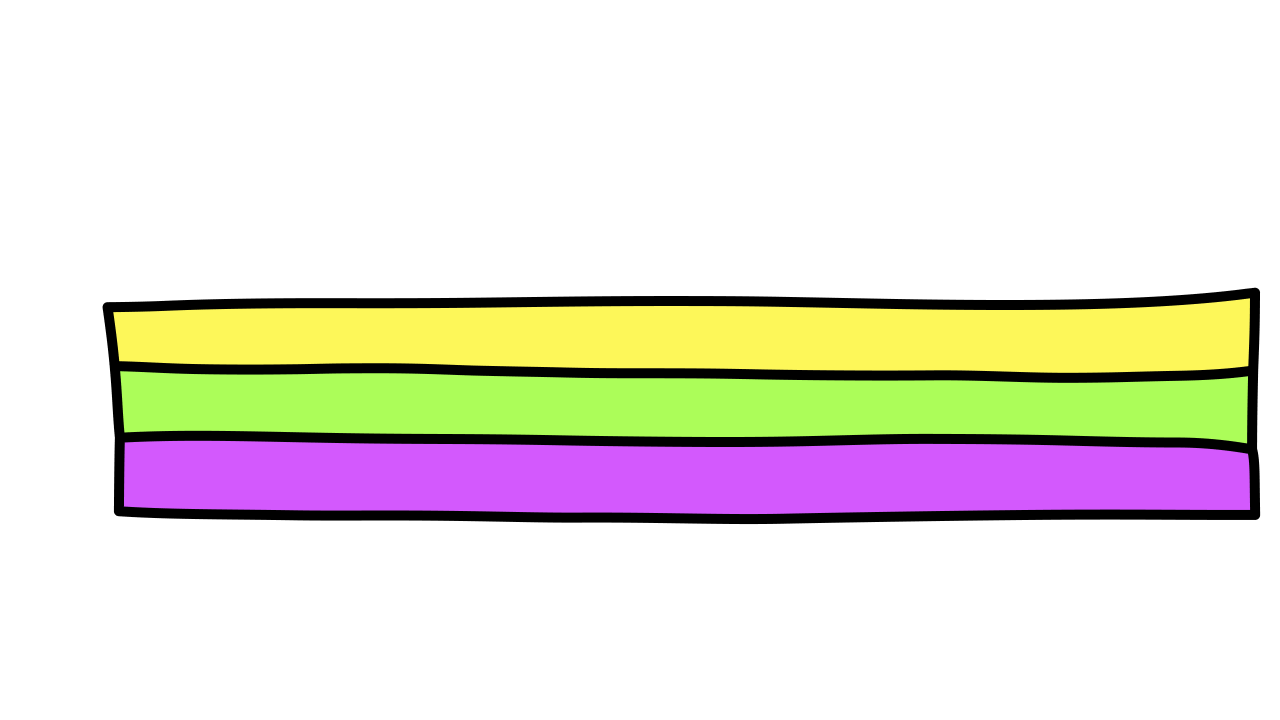
\includegraphics[scale=0.2]{unFoldDescription1.png}
	\caption{Un-Fold example. Ending Configuration}
    \end{minipage}
\end{figure}
\textbf{Precondition:} there are no preconditions for this event. the user is free to play with this event as it allows geologists to test their hypothesis on forces that have been applied to the section in the past.\\\\
\textbf{Simulation:} We add external forces either to a block, a unit or a specific mass during the requested time. The external forces are taken into account in the main physical loop.\\\\
\textbf{Duration:} given by the user.\\\\
\textbf{Postcondition:} The event no longer apply forces on the concerned particles.\\\\

\section{Un-Fault}

Here we will describe the un-fault event which has special feature of being a composed event. Indeed we consider the un-fault event as being composed of three events: un-erode, un-slide and un-fold. As an un-fault event can only occur between two blocks (and only two) we will proceed by first un-eroding units which are not in contact and then making one block sliding on the other while un-folding the whole cross-section. We can note that when an fault occur, it breaks one block starting by the oldest layer to the youngest. We will use this property to decompose our un fault event into several stickUnits events for units we don't un-erode at the beginning of the un-fault event.\\\\
% dessin
\begin{figure}[h]
    \begin{minipage}[c]{.46\linewidth}
        \centering
        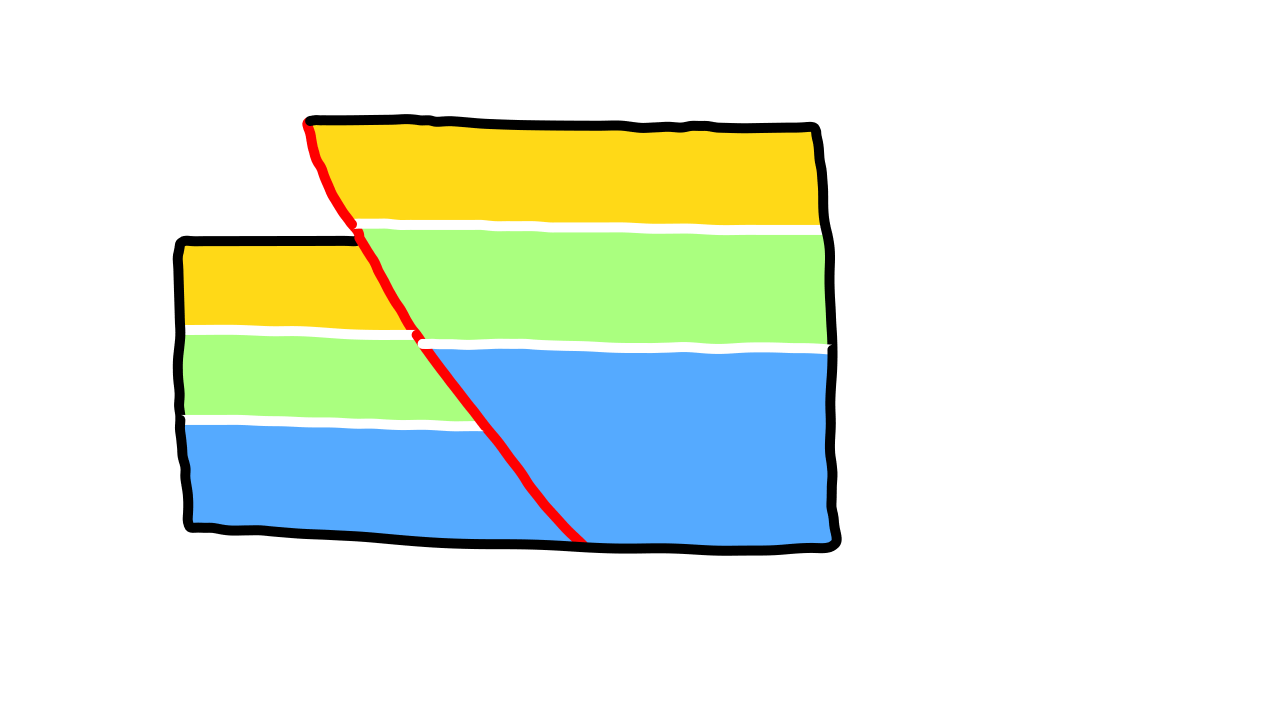
\includegraphics[scale=0.2]{unFaultDescription0.png}
	\caption{Un-Fault example. Starting Configuration}
    \end{minipage}
    \hfill%
    \begin{minipage}[c]{.46\linewidth}
        \centering
        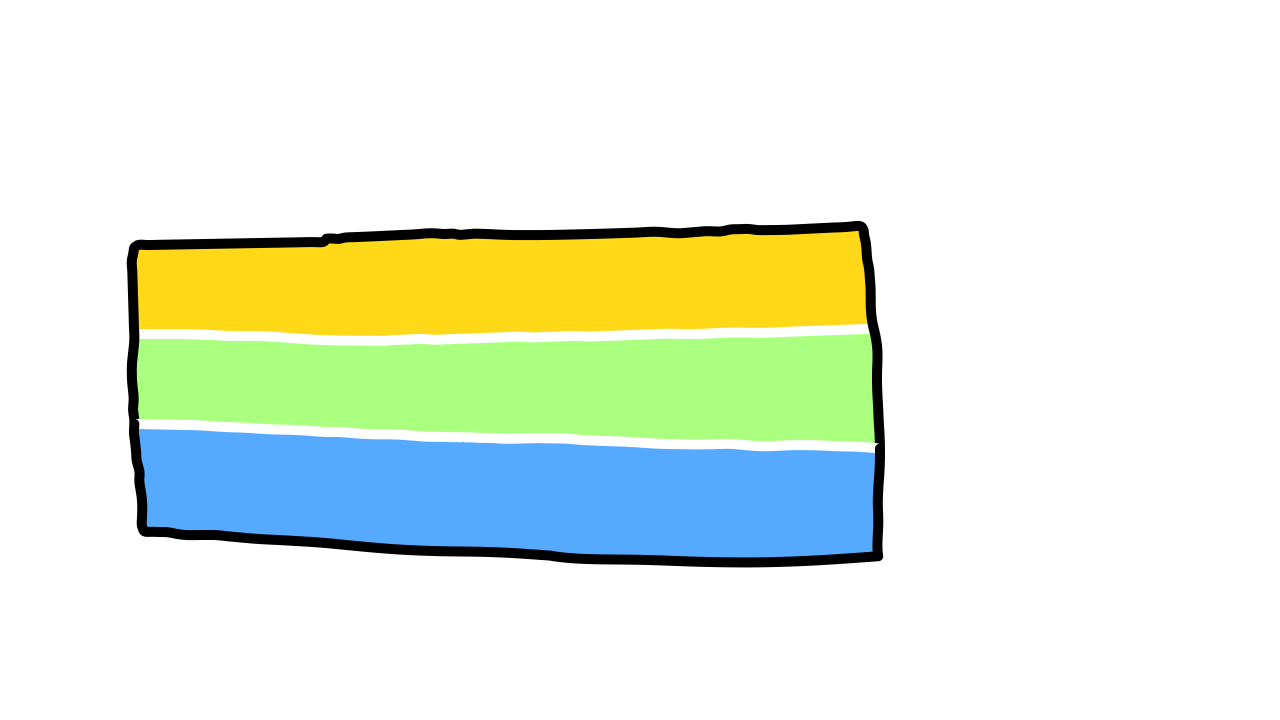
\includegraphics[scale=0.2]{unFaultDescription1.png}
	\caption{Un-Fault example. Ending Configuration}
    \end{minipage}
\end{figure}
Before explaining the un-fault event, we will present the simple stickUnit event. There are no preconditions has it is the created and called by the fault event which manage preconditions. This event wait for matching unit to be face to face and merge them when there are. In addition as fault can be created by extreme folding condition we apply an little attraction force on the sliding unit in order to fold it like it was at the moment of the break. Thus we apply $\overrightarrow{F} = d*\frac{\overrightarrow{(C_{lower} - C_{upper})} }{||\overrightarrow{(C_{lower} - C_{upper})}||}$ to the corners of the sliding unit going toward the corresponding corners of the matching unit.\\\\
We can now detail the un-fault event.\\\\
\textbf{Precondition:} The fault must be between two blocks and only two of them.\\\\
\textbf{Simulation:} We first ask the user if he wants to un-erode units which are not in contact in the fault using the "Un-Erode two facing units of the same Material" algorithm we describe before. Then we create the stickUnits event for each matching unit, they will be simulated one after the other starting by the youngest units to the oldest. At the same time we will let one block to slide on the other (the upper one in the case of the compression, the lower one if it is an extension) and fold on one extremity of the cross section depending if we are in a compression or extension and depending the direction of folding. This event ends when all the stick events have also ended.\\\\
\textbf{Postcondition:} all the sticking events ended meaning that all matching units merged together one new unit. That implies that the two concerned blocks merged.\\\\
\textbf{Postcomputation:} regenerate the mass-spring system of the containing block at the end of the event for a better mesh uniformity.\\\\ 
	

\chapter{Cross section analysis}

As mentionned above our input drawing will be built using vpaint software which implements the VAC and VGC structures (refs).
More preciselly we will use a VGC as input which is composed of vertices, edges and faces. This choice is justified by the fact that VGC can model all possible incidence relations between faces in 2D sketches and our cross-section is composed only of adjacent faces. An interesting feature of these structures is that each instance has a unique identifier and color which will allow us to build our geological structure.\\\\
Here is an exemple of an input cross section using vpaint:
%chartreuse section

 \begin{figure}[H]
	\centering
	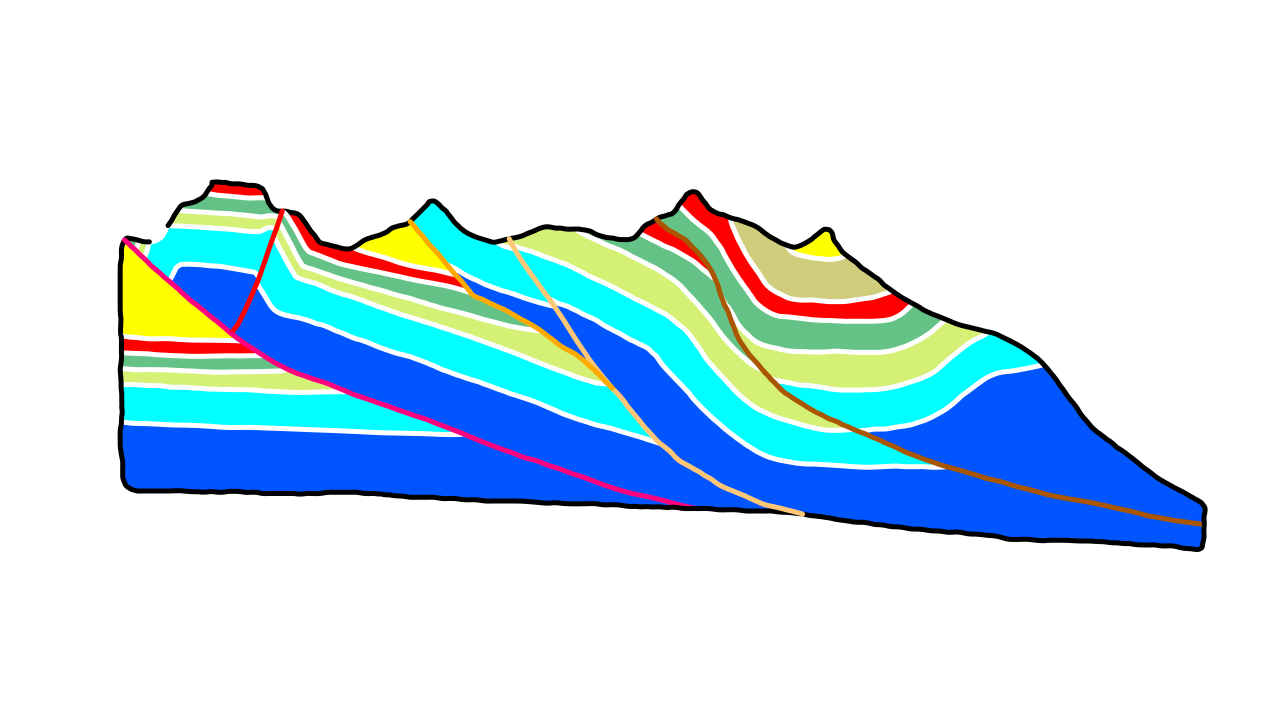
\includegraphics[scale=0.5]{chartreusevpaint.png}
	\caption{Chartreuse section drawn with VPaint}
\end{figure}

We will use the precendently described geological structure as our intern cross section data structure. In other words a drawing will be represented as a cross section which will be composed of blocks themselves composed of units. Because we consider that at the restoration state all units are straight rectangles, we decompose our units into two sides (left and right) and two level boundaries (upper and bottom) which either make the links between unit or constitute the limits of the drawing. 
%drawing

 \begin{figure}[H]
	\centering
	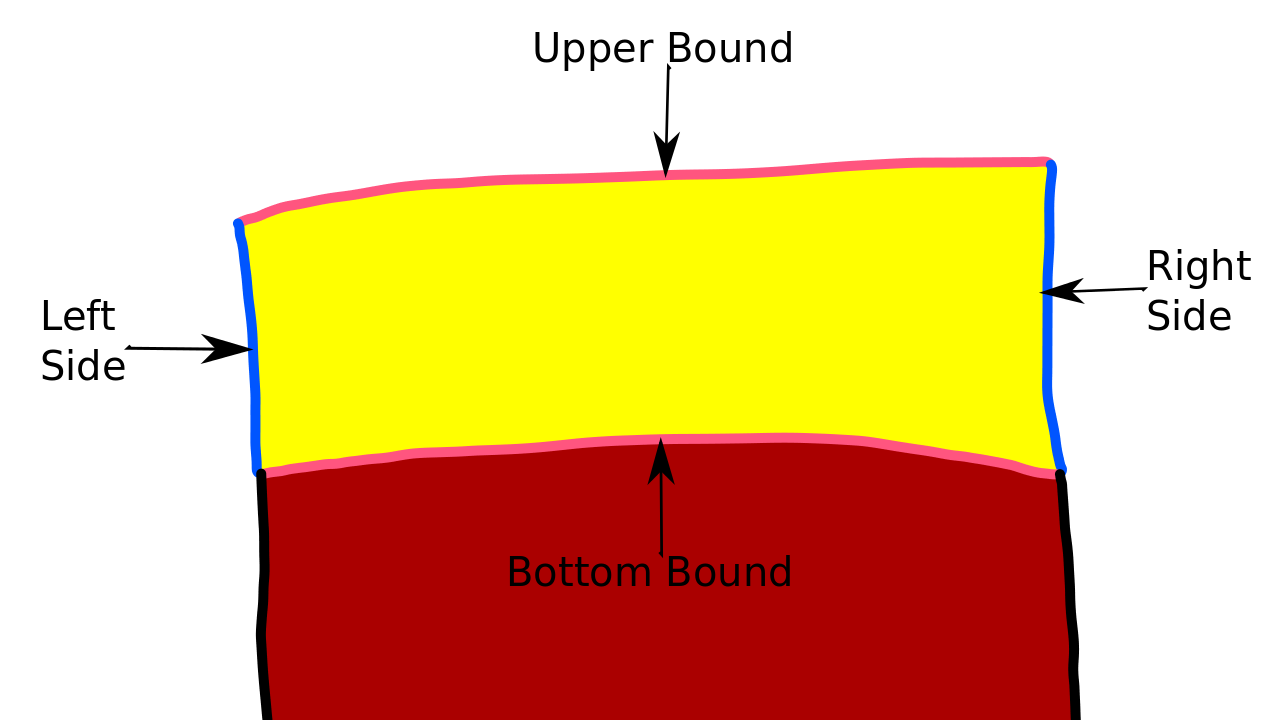
\includegraphics[scale=0.3]{unitDescriptionEdit.png}
	\caption{Geological unit representation}
\end{figure}

Thus we must deduce those structure from the input vpaint file. \\\\\
To do so we use the colors of our edges and faces. When importing the drawing we first ask to the user to give the different time period for each material exisiting in the cross section. Then we will build our blocks by adding succefully all the unit of each layer starting the youngest ones to the oldest. We do this sort in order to simplify the block creation and minimize the number of block created during this phase. Moreover when adding a new unit we try to find one already added unit which share either one portion of its upper bound  or its bottom bound with it. If we can't find one matching unit we place it in a new block. If we find one or several sharing units we deduce that they are all part of the same block so we store them in one unique block. If we do the sort like previously enonced we will thus reduce the number of block created because the only cases where we create blocks are either when the newly added unit is a surface unit or is unit located in a different block than the previously added ones.\\\\

When we have all our blocks created in our internal stucture we can identify the fault by looking at the color of the edges. If it is different than black or wite then it correspond to a fault which are caractarised by they color. The units are caracterized by their face color and their upper and bottom bounds which are drawn in white for most of them. Cross section border are usually drawn in black but we can deduce automatically which edge belongs to the lacking bound (limitation it is not always good).\\\\

We then have all the different material age, the blocks and units objects and the different fault we can find in the drawing. We will store all these information into a configuaration file .geo which will allow the user to save time by not giving the material information each times he opens the file. We have to note that in the input XML file, faces have an arbitrary cycling orientation which can be clockwise or counterclockwise. That's why but for building and manipulating our structure more easelly we will choose the convention that all our units will be first read clockwiselly. Thus we reverse the faces which are written counterclockwisely\\\\
 
 
\chapter{Implementation}

Almost every parts of our geological tool has been implemented in C++. We propose a Qt OpenGL interface where the user can load vec files or geo files which are configuration files created after reading a vec file which store additionnal information entered by the user when he openned the corresponding vec file. It is time saving for users who don't want to enter several times the same additionnal information for  given a cross section. \\\\
We implemented our tool using both geological stucture and the parts of VGC one. We used the base structure of VGC such as \textbf{Vertex}, \textbf{Edge} and \textbf{Face} inheriting from \textbf{Cell} which possesses an attribute \textbf{Id} allowing to identify a instance uniquely. This feature is important for manipulating this structures which will be encompassed in our geological framework. Indeed as we implemented our geological data structure following cross sections' organisation we need identtification information for our units, blocks and faults.\\\\
To be more accurate we implemented the cross-section structure in a hierarchical way: the \textbf{Crosssection} class contains a vector of \textbf{Block} containing a vector of \textbf{Unit} which possesses a \textbf{MassSpringSystem}. In addition this hierarchy is a two way one, meaning that each member of the hierarchy has access to its parent.\\\\
The story telling part has also been implemented and represents the most generic part because it is templated and can be used directly with any context other than geology. The \textbf{Story Graph} is a \textbf{Graph} of \textbf{Story Node} with \textbf{Story Egde}. Like we presented it in section ... a \textbf{Story Node} contains a list of simulable events and a \textbf{Story Edge} contains the list of events to be simulated choosen by the user.
Due to lack of time, the event proposition and selection user interface is limited to a terminal screening and the user can only simulate one event for each proposition. As for the \textbf{Event Graph}, it has also been implemented and contains \textbf{Event Nodes} which represents one event\\\\
The \textbf{Event} class is an abstract class containing all the feature we used to describe our geological event in section ... such as functions to check if the precondition and postcondition have been fulfilled and the simulate function.\\\\
The Implicit Euler Scheme has been implemented like described in section ... in the \textbf{MassSpringSystem} class instanciated in each \textbf{Unit}.\\\\
Finally all the un-do function for each geological events have been implemented in each geological event class and uses functions provided by our geological API such as \textbf{MergeTwoUnits(Unit1,Unit2)}. 

\chapter{Results}
We ran our system over several examples including unit tests which show how we simulate each geological events.
Our main example we wanted to solve is the Chartreuse cross section which is a good complex example because it underwent lots of geological events. This is example allow us also to validate our model because we were provided the restoration event sequence by geologist who were able to recover the whole history of the cross-section. Thus if our system detect this sequence as a path in our Story Graph and if our simulation gives a convincing result by comparing with the provided restoration we will have a validation for our model.\\\\
We will first present our results on several of our unit tests showing how our system works on simple example and then present the Chartreuse restoration with two different scenarios, one being the geologist provided sequence.\\\\\

\chapter{Limitations}

- 3D with more Cross sections\\
- Could have used clothoid for preserving layer thickness\\
- Sequential and not list of un-doing events\\
- Let the user draw erosion line -- already determined eroded zones\\
- Thickness limitation: it is not geologicaly good because we don't look at the layer thickness.

\chapter{Conclusion}
The main goal of this work was to investigate a new geological cross section restoration method which allows users to explore multiple scenarios in real time way. 
In order to achieve this goal we proposed to use mass-spring systems as a base of our animation because of the fast computation time they require. We showed that they are sufficient to procude convincing animations validated by geologists. Moreover 


\chapter{Annex}

Hermite curves equations :\\
Given two points $P_0, P_1$ and two tangents $T_0, T_1$ being the tangent we can find at the matching number points, the Hermite interpolation which will produce a $C_1$ curve has for equation : 


\begin{equation}
h(t) = (2*t^3 - 3*t^2 + 1)*P_0 + (t^3 - 2*t^2 + t)*T_0 + (t^3 -t^2)*T_1 +(3*t^2 - 2*t^3)*P_0
\end{equation}

It is possible to multiply the tangent by a bias factor which will make the curvature of the curve varying more when this factor becomes big.\\\\\

Collisions methods: \\
%TODO add friction
Collisions between blocks. Each layer is delimited by its boundaries which we devide into four parts: upper interlayer, bottom interlayer, right side and left side. Each of these part are composed of segments and the union of all of them is a closed polygon. We deal with block collision by computing particle (circle) segments collision. Moreover for each particle of one block we consider the segement built by the particle position at time $t - dt$ and its position at time $t$ and we check if this segment crosses one of the other blocks segment border. In addition, with this we can also check for collision inside the block it self which is usefull to give reallistic results for un sedimentation for instance. This technique as the advantage of determinig precisely the segment with which the particle collided even if the particle went through the colliding block. However there is still a chance to fail at identifying a collision depending on the order we treat each block animation and collision detection.\\
In order to check intersection between segments we proceed the following way:\\
Given two sgements $[PQ]$ and $[RS]$ we will consider a parametrisation of their equations: 

\begin{align}
	PQ &= P + t*\overrightarrow{PQ} \forall t \in [0,1]\\
	RS &= R + u*\overrightarrow{RS} \forall u \in [0,1]\\
\end{align}

With this parametrisation the two segments intersect if and only if:\\
\begin{equation}
\exists t,u \in [0,1], P + t*\overrightarrow{PQ} = R + u*\overrightarrow{RS}
\end{equation}


We need to extract two equations from this one in order to find $u$ and $t$.
To do so we will use the cross product to keep only one variable in each equation. Thus by applying a cross product with $\overrightarrow{PQ}$ and $\overrightarrow{RS}$ we obtain the following equations:

\begin{align}
	t &= \frac{\overrightarrow{(R - P)} \wedge \overrightarrow{RS}}{\overrightarrow{PQ} \wedge \overrightarrow{RS}}\\
	u &= \frac{\overrightarrow{(P - R)} \wedge \overrightarrow{PQ}}{\overrightarrow{RS} \wedge \overrightarrow{PQ}}
\end{align}

We must note that the simplification was made by noticing that $\overrightarrow{PQ} \wedge \overrightarrow{PQ} = 0$ and $\overrightarrow{RS} \wedge \overrightarrow{RS} = 0$.

Then we can distinguish $4$ cases :\\\\
1) $ \overrightarrow{RS} \wedge \overrightarrow{PQ} = 0$ and $\overrightarrow{(P - R)} \wedge \overrightarrow{PQ} = 0$\\\\
This means that our segments are parrallel because of the first condition and colinear because of the second. We deduce that our segement are intersecting if: \\\\ 
($\overrightarrow{PR}.\overrightarrow{PS} < 0$) or ($\overrightarrow{PR}.\overrightarrow{PS} \geq 0$ and $\overrightarrow{PQ}.\overrightarrow{PS} \geq 0$ and ($||\overrightarrow{PS}|| < ||\overrightarrow{PQ}||$ or $||\overrightarrow{PR}|| < ||\overrightarrow{PQ}||$))
\\\\\
2)  $ \overrightarrow{RS} \wedge \overrightarrow{PQ} = 0$ and $\overrightarrow{(P - R)} \wedge \overrightarrow{PQ} \neq 0$
In that case the segeents are parallel but non intersecting.\\\\
3)  $ \overrightarrow{RS} \wedge \overrightarrow{PQ} \neq 0$.
The segment are intersecting iff the computation of $t$ and $u$ gives $t,u \in [0,1]$\\\\
4) Otherwise the segements are not parallel and non intersecting\\\\



\bibliography{pfe.bib}
\end{document} 